% ==========================================================================
% Rapport de Projet --- Systeme d'Inspection Visuelle de Stators
% Version Recherche Academique --- avec references bibliographiques completes
% ==========================================================================
\documentclass[12pt,a4paper]{report}

% --- Encodage et langue ---------------------------------------------------
\usepackage[utf8]{inputenc}
\usepackage[T1]{fontenc}
% \usepackage[french]{babel}  % Uncomment when texlive-lang-french is installed
% --- Traductions manuelles (remplacement de Babel) ---
\renewcommand{\contentsname}{Table des mati\`eres}
\renewcommand{\chaptername}{Chapitre}
\renewcommand{\figurename}{Figure}
\renewcommand{\tablename}{Tableau}
\renewcommand{\appendixname}{Annexe}
\renewcommand{\bibname}{Bibliographie}
\def\today{16 Avril 2026}

% --- Mise en page ---------------------------------------------------------
\usepackage[margin=2.5cm]{geometry}
\usepackage{setspace}
\onehalfspacing

% --- Typographie et couleurs ----------------------------------------------
\usepackage{lmodern}
\usepackage{xcolor}
\definecolor{primaryblue}{HTML}{2C5F8A}
\definecolor{accentgreen}{HTML}{1A8A4A}
\definecolor{alertred}{HTML}{CC4444}
\definecolor{sectioncolor}{HTML}{483D8B}

% --- Images et figures ----------------------------------------------------
\usepackage{graphicx}
\usepackage{float}
\usepackage{subcaption}
\usepackage{wrapfig}

% --- Tableaux -------------------------------------------------------------
\usepackage{booktabs}
\usepackage{longtable}
\usepackage{tabularx}
\usepackage{multirow}
\usepackage{array}

% --- Liens et references -------------------------------------------------
\usepackage{hyperref}
\hypersetup{
    colorlinks=true,
    linkcolor=primaryblue,
    urlcolor=primaryblue,
    citecolor=accentgreen,
}

% --- Titres personnalises -------------------------------------------------
\usepackage{titlesec}
\titleformat{\chapter}[display]
    {\normalfont\huge\bfseries\color{sectioncolor}}
    {\chaptertitlename\ \thechapter}{20pt}{\Huge}
\titleformat{\section}
    {\normalfont\Large\bfseries\color{primaryblue}}
    {\thesection}{1em}{}
\titleformat{\subsection}
    {\normalfont\large\bfseries\color{sectioncolor}}
    {\thesubsection}{1em}{}

% --- En-tete et pied de page ---------------------------------------------
\usepackage{fancyhdr}
\pagestyle{fancy}
\fancyhf{}
\fancyhead[L]{\small\textit{Rapport de Projet --- Inspection Visuelle de Stators}}
\fancyhead[R]{\small\thepage}
\fancyfoot[C]{\small\textcolor{gray}{Confidentiel --- Usage Interne}}
\renewcommand{\headrulewidth}{0.4pt}

% --- Divers ---------------------------------------------------------------
\usepackage{enumitem}
\usepackage{amsmath}
\usepackage{microtype}


% ==========================================================================
\begin{document}

% --- Page de garde --------------------------------------------------------
\begin{titlepage}
    \centering

    % --- Logos entreprise ---
    \vspace*{0.5cm}
    \begin{figure}[H]
        \centering
        
\includegraphics[height=2cm]{logos/nextronic.png}
        \hspace{2cm}
        
\includegraphics[height=2cm]{logos/aba_technology.png}
    \end{figure}
    \vspace{1cm}

    \rule{\textwidth}{1.5pt}\\[0.4cm]
    {\Huge\bfseries\color{sectioncolor} Syst\`eme d'Inspection Visuelle\\[0.3cm] de Stators par Intelligence Artificielle}\\[0.3cm]
    \rule{\textwidth}{1.5pt}\\[1.5cm]

    {\Large\textbf{Rapport de Projet}}\\[0.5cm]
    {\large\textit{De l'entra\^inement des mod\`eles \`a la d\'etection en temps r\'eel}}\\[2cm]

    \begin{tabular}{ll}
        \textbf{Auteur :}    & Youssef MAHDI \\
        \textbf{Encadrant :} & Zakaria ABOUHANIFA \\
        \textbf{Entreprise :}& Nextronic, ABA Technology \\
        \textbf{Date :}      & \today \\
    \end{tabular}

    \vfill
\end{titlepage}

% --- Table des mati\`eres ---------------------------------------------------
\tableofcontents
\newpage

% ==========================================================================
\chapter{Introduction}
% ==========================================================================

\section{Contexte du projet}

Dans le cadre de l'industrie 4.0, l'inspection visuelle automatis\'ee des composants \'electrom\'ecaniques repr\'esente un enjeu majeur pour le contr\^ole qualit\'e. Les m\'ethodes classiques d'inspection reposent sur des op\'erateurs humains sujets \`a la fatigue et \`a la variabilit\'e, ce qui justifie le recours aux syst\`emes de vision par ordinateur fond\'es sur l'apprentissage profond (\textit{deep learning}). Ce projet vise \`a d\'evelopper un syst\`eme complet d'inspection visuelle de \textbf{stators de moteurs \'electriques} utilisant des techniques avanc\'ees de segmentation d'instances et de classification.

La segmentation s\'emantique et par instances constitue l'une des t\^aches les plus exigeantes de la vision par ordinateur~: il s'agit d'assigner une \'etiquette de classe \`a chaque pixel de l'image, tout en distinguant les instances individuelles au sein d'une m\^eme classe. Depuis les r\'eseaux enti\`erement convolutifs (FCN) de Long \textit{et al.}~\cite{long2015fcn} et l'architecture U-Net de Ronneberger \textit{et al.}~\cite{ronneberger2015unet}, l'\'etat de l'art a consid\'erablement \'evolu\'e, notamment gr\^ace aux architectures \`a base de Transformeurs~\cite{xie2021segformer}.

Le syst\`eme d\'evelopp\'e dans ce rapport est con\c{c}u pour d\'etecter et mesurer trois cat\'egories de composants critiques sur un stator :
\begin{itemize}[leftmargin=2cm]
    \item \textbf{Cercle} --- Le contour principal circulaire du stator
    \item \textbf{Aimants} --- Les p\^oles magn\'etiques (2 par stator, positionn\'es aux angles cardinaux)
    \item \textbf{Pi\`eces m\'ecaniques} --- Les fixations structurelles diagonales (4 par stator)
\end{itemize}

Le projet couvre \'egalement deux domaines suppl\'ementaires :
\begin{itemize}[leftmargin=2cm]
    \item \textbf{Chignon} --- D\'etection des bobinages de cuivre (chignons), composants sensibles \`a la d\'eformation
    \item \textbf{Files (c\^ables)} --- Classification et validation de la position des c\^ables color\'es (bleu/jaune) selon un ordre gauche-droite normalis\'e
\end{itemize}

\section{Objectifs}
\begin{enumerate}
    \item D\'evelopper un pipeline d'entra\^inement complet avec augmentation de donn\'ees industrielle \`a fort facteur de multiplication
    \item Entra\^iner et comparer plusieurs architectures de segmentation : U-Net~\cite{ronneberger2015unet} avec encodeur ResNet-18~\cite{he2016resnet}, SegFormer~\cite{xie2021segformer}, DeepLabV3~\cite{chen2017deeplabv3} et les familles YOLO~\cite{jocher2023yolov8}
    \item Cr\'eer une application web temps r\'eel avec WebRTC pour l'inf\'erence \textit{live}
    \item Impl\'ementer un syst\`eme de mesure g\'eom\'etrique (px $\rightarrow$ mm) avec calibration, incluant l'estimation de profondeur monoculaire par MiDaS~\cite{ranftl2020midas}
    \item D\'eployer l'ensemble via Docker avec suivi d'exp\'eriences MLflow
\end{enumerate}

\section{Technologies utilis\'ees}
\begin{table}[H]
\centering
\begin{tabular}{ll}
\toprule
\textbf{Composant} & \textbf{Technologies} \\
\midrule
Backend         & Flask, Python 3.11, WebRTC \\
Frontend        & HTML5, JavaScript, Canvas API \\
Mod\`eles IA      & PyTorch, Ultralytics YOLO~\cite{jocher2023yolov8}, ONNX Runtime \\
Augmentation    & OpenCV, Copy-Paste~\cite{ghiasi2021copypaste} \\
Fonctions de perte & BCE, Dice, Boundary~\cite{kervadec2019boundary}, Lov\'asz~\cite{berman2018lovasz} \\
Suivi d'objets  & ByteTrack~\cite{zhang2022bytetrack} \\
D\'eploiement     & Docker, Docker Compose, Nginx \\
Suivi           & MLflow \\
Cam\'era          & MindVision SDK, WebRTC MediaStream \\
\bottomrule
\end{tabular}
\caption{Stack technologique du projet}
\end{table}


% ==========================================================================
\chapter{Architecture du Syst\`eme}
% ==========================================================================

\section{Vue d'ensemble de l'architecture}

L'architecture du syst\`eme suit un mod\`ele client-serveur multi-domaine, orchestr\'e par Docker Compose avec trois services principaux. La figure~\ref{fig:multi_domain} illustre le routage des requ\^etes depuis le client web jusqu'aux modules de domaine sp\'ecialis\'es.

Le choix d'une architecture multi-domaine r\'epond \`a une exigence fondamentale : chaque domaine d'inspection (stator, chignon, c\^ables) pr\'esente des caract\'eristiques visuelles tr\`es diff\'erentes, ce qui justifie des pipelines de post-traitement et des strat\'egies d'inf\'erence d\'edi\'es. Cette s\'eparation des responsabilit\'es s'inspire des principes de \textit{microservices}, o\`u chaque composant est ind\'ependant, testable et rempla\c{c}able.

\begin{figure}[H]
    \centering
    
\includegraphics[width=0.50\textwidth]{multi_domain_architecture.png}
    \caption{Architecture multi-domaine --- Routage des requ\^etes vers les modules sp\'ecialis\'es (Stator, Chignon, File) via le serveur central.}
    \label{fig:multi_domain}
\end{figure}

\section{Architecture Docker}

Le d\'eploiement repose sur trois conteneurs Docker isol\'es, garantissant la reproductibilit\'e de l'environnement d'ex\'ecution.

\subsection{Service Serveur (Backend IA)}

Le serveur principal h\'eberge le backend d'inf\'erence et le point de terminaison WebRTC. Il fonctionne sur une image Python l\'eg\`ere, avec acc\`es au GPU NVIDIA pour l'acc\'el\'eration mat\'erielle des mod\`eles de deep learning. Il expose un port unique pour toutes les interactions (API REST et WebRTC) et v\'erifie sa disponibilit\'e via un m\'ecanisme de contr\^ole de sant\'e automatique.

\subsection{Service MLflow}

MLflow est un framework open-source de gestion du cycle de vie des mod\`eles d'apprentissage automatique. Il permet de journaliser les hyperparam\`etres, les m\'etriques et les art\'efacts de mod\`ele de mani\`ere structur\'ee et reproductible. Dans ce projet, MLflow est int\'egr\'e \`a deux niveaux~:
\begin{enumerate}
    \item \textbf{Entra\^inement} --- Journalisation des hyperparam\`etres, m\'etriques par \'epoque, et art\'efacts de mod\`ele
    \item \textbf{Inf\'erence} --- Sessions r\'esum\'ees (FPS moyen, latence, nombre de d\'etections) journalis\'ees automatiquement
\end{enumerate}

\subsection{Service Client (Proxy inverse)}

Le troisi\`eme service est un serveur web l\'eger (Nginx) servant les fichiers statiques de l'application web et jouant le r\^ole de proxy inverse vers le backend. Cette s\'eparation permet de servir efficacement les ressources statiques et de router les requ\^etes API de mani\`ere transparente.

\section{Communication temps r\'eel (WebRTC)}

Le protocole WebRTC (Web Real-Time Communications) permet d'\'etablir des connexions pair-\`a-pair directement dans le navigateur, sans plugin externe. Le pipeline de traitement vid\'eo temps r\'eel fonctionne comme suit~:
\begin{enumerate}
    \item R\'eception du flux vid\'eo depuis la cam\'era du navigateur
    \item Conversion de chaque trame en image pour le traitement
    \item Ex\'ecution de l'inf\'erence via le module de domaine s\'electionn\'e
    \item Renvoi de la trame annot\'ee vers le navigateur
    \item Transmission des r\'esultats structur\'es (JSON) via un canal de donn\'ees d\'edi\'e, avec une latence typiquement inf\'erieure \`a 50\,ms
\end{enumerate}

\section{Syst\`eme multi-domaine}

Un routeur de domaine dirige chaque requ\^ete vers le module d'inf\'erence appropri\'e~:
\begin{itemize}
    \item \textbf{Module Stator} --- Supporte YOLO et les mod\`eles PyTorch, g\`ere 4 classes de composants, int\`egre le moteur de mesures g\'eom\'etriques compl\`etes
    \item \textbf{Module Chignon} --- Supporte YOLO et UNet~\cite{ronneberger2015unet}, segmentation binaire (fond vs. chignon)
    \item \textbf{Module Files} --- Utilise exclusivement UNet~\cite{ronneberger2015unet}, enrichi par une classification couleur dans l'espace HSV
\end{itemize}


% ==========================================================================
\chapter{Pr\'eparation des Donn\'ees}
% ==========================================================================

\section{Format des annotations}

Les images sont annot\'ees au format \textbf{LabelMe} (JSON), un outil d'annotation open-source d\'evelopp\'e par le MIT CSAIL. Trois types de formes g\'eom\'etriques sont support\'es~:
\begin{itemize}
    \item \textbf{Polygone} --- Contour ferm\'e standard repr\'esentant une r\'egion
    \item \textbf{Polyligne} --- S\'equence de points ouverte, ferm\'ee automatiquement par le pipeline
    \item \textbf{Segment} --- Paire de 2 points, convertie en rectangle fin pour g\'erer les fixations filiformes
\end{itemize}

Le pipeline de chargement des donn\'ees r\'ealise les op\'erations suivantes~:
\begin{enumerate}
    \item Chargement des paires image / fichier d'annotation
    \item G\'en\'eration des masques multi-classes \`a partir des formes annot\'ees
    \item Redimensionnement \`a la taille cible ($512 \times 512$ pixels) par interpolation bilin\'eaire
    \item Application du mapping de classes~: arri\`ere-plan, pi\`ece m\'ecanique, aimant, cercle
\end{enumerate}

\section{Division du jeu de donn\'ees}

La r\'epartition est r\'ealis\'ee de mani\`ere d\'eterministe, conform\'ement aux bonnes pratiques d'apprentissage automatique pour assurer la reproductibilit\'e~:
\begin{itemize}
    \item \textbf{70\,\%} --- Entra\^inement : maximise le volume de donn\'ees d'apprentissage
    \item \textbf{15\,\%} --- Validation : guide l'arr\^et pr\'ecoce et la s\'election des hyperparam\`etres
    \item \textbf{15\,\%} --- Test : \'evaluation finale non biais\'ee des performances
\end{itemize}

Ce ratio 70/15/15, classique dans la litt\'erature, permet un compromis entre la richesse du jeu d'entra\^inement et la fiabilit\'e de l'\'evaluation dans des r\'egimes de donn\'ees de taille modeste, typiques des applications industrielles sp\'ecialis\'ees.

\section{Pipeline d'augmentation de donn\'ees}

L'augmentation de donn\'ees est une technique essentielle pour am\'eliorer la g\'en\'eralisation des mod\`eles, en particulier lorsque les jeux de donn\'ees industriels sont de taille limit\'ee. Le pipeline d'augmentation proc\`ede en deux \'etapes, produisant un facteur de multiplication total de $5 \times 9 = 45\times$ par image originale.

\subsection{Transformations g\'eom\'etriques ($5\times$)}

Chaque transformation est appliqu\'ee de mani\`ere coh\'erente~: les coordonn\'ees des annotations polygonales sont mises \`a jour par transformation affine pour rester align\'ees avec les pixels transform\'es.
\begin{enumerate}
    \item Identit\'e (image originale)
    \item Retournement horizontal
    \item Rotation $90^{\circ}$ horaire
    \item Rotation $180^{\circ}$
    \item Rotation $270^{\circ}$ horaire
\end{enumerate}

Les rotations de $90^{\circ}$, $180^{\circ}$ et $270^{\circ}$ sont particuli\`erement pertinentes pour les stators, dont la g\'eom\'etrie pr\'esente une sym\'etrie de r\'evolution~: un stator peut en effet \^etre mont\'e dans quatre orientations.

\subsection{Transformations photom\'etriques ($9\times$)}

Ces transformations simulent les variations d'\'eclairage rencontr\'ees en milieu industriel (\'eblouissement, sous-exposition, vieillissement des capteurs)~:
\begin{enumerate}
    \item Original (sans modification)
    \item Luminosit\'e augment\'ee
    \item Luminosit\'e diminu\'ee
    \item Contraste augment\'e
    \item Flou gaussien --- simule les flous de mouvement ou de mise au point
    \item CLAHE (\textit{Contrast Limited Adaptive Histogram Equalization}) --- normalisation locale du contraste
    \item Correction gamma sombre --- simulation de sous-exposition
    \item Correction gamma clair --- simulation de sur-exposition
    \item D\'ecalage de luminosit\'e HSV --- variation de teinte sous \'eclairage artificiel
\end{enumerate}

\subsection{Copy-Paste Augmentation (SOTA)}

La m\'ethode \textit{Simple Copy-Paste}~\cite{ghiasi2021copypaste}, propos\'ee par Ghiasi \textit{et al.} (CVPR 2021), constitue une avanc\'ee majeure dans l'augmentation pour la segmentation d'instances. Le principe consiste \`a~:
\begin{itemize}
    \item Extraire des instances segment\'ees (objets individuels avec leurs masques) depuis des images source
    \item Les coller avec canal alpha sur des images cible choisies al\'eatoirement
    \item Appliquer une mise \`a l'\'echelle al\'eatoire ($0.5\times$ \`a $1.5\times$) pour varier les tailles apparentes
    \item Mettre \`a jour automatiquement les annotations pour refl\'eter les nouvelles positions
\end{itemize}

Ghiasi \textit{et al.} ont d\'emontr\'e sur MS-COCO qu'un collage al\'eatoire sans mod\'elisation du contexte est suffisant pour obtenir des gains significatifs (+0.6 mask AP et +1.5 box AP). Cette approche est particuli\`erement bien adapt\'ee au contexte industriel o\`u les stators apparaissent toujours sur des fonds d'atelier relativement uniformes.

\textbf{Facteur de multiplication total :} $5 \times 9 = 45\times$ par image + Copy-Paste

\section{Conversion au format YOLO}

Les annotations au format LabelMe sont \'egalement converties au format YOLO segmentation (coordonn\'ees normalis\'ees dans $[0, 1]$), ce qui permet d'exploiter directement l'\'ecosyst\`eme Ultralytics YOLO~\cite{jocher2023yolov8} pour l'entra\^inement des mod\`eles de d\'etection d'instances.


% ==========================================================================
\chapter{Pipeline d'Entra\^inement}
% ==========================================================================

\begin{figure}[H]
    \centering
    
\includegraphics[width=0.50\textwidth]{training_pipeline.png}
    \caption{Pipeline d'entra\^inement complet en six phases : donn\'ees brutes, augmentation, conversion de format, architectures de mod\`eles, boucle d'entra\^inement, et \'evaluation/sortie. Les deux branches (Ultralytics YOLO et PyTorch personnalis\'e) partagent les m\^emes donn\'ees augment\'ees.}
    \label{fig:training_pipeline}
\end{figure}

\section{Architectures de mod\`eles}

\subsection{U-Net avec encodeur ResNet-18}

L'architecture U-Net~\cite{ronneberger2015unet}, introduite par Ronneberger \textit{et al.} (MICCAI 2015), constitue le mod\`ele de r\'ef\'erence pour la segmentation s\'emantique dense. Sa structure sym\'etrique encodeur-d\'ecodeur avec connexions de saut (\textit{skip connections}) permet de combiner des informations s\'emantiques profondes avec des d\'etails spatiaux fins.

Dans cette impl\'ementation, l'encodeur U-Net standard est remplac\'e par un \textbf{ResNet-18 pr\'e-entra\^in\'e}~\cite{he2016resnet}. ResNet (He \textit{et al.}, CVPR 2016) introduit des connexions r\'esiduelles qui permettent d'entra\^iner des r\'eseaux tr\`es profonds en \'evitant le probl\`eme de la disparition du gradient. La formule de base est~:
\[
    \mathbf{y} = \mathcal{F}(\mathbf{x}, \{W_i\}) + \mathbf{x}
\]
o\`u $\mathcal{F}$ repr\'esente la transformation \`a apprendre et $\mathbf{x}$ le raccourci d'identit\'e. L'encodeur ResNet-18, pr\'e-entra\^in\'e sur ImageNet, fournit des repr\'esentations robustes des textures et structures visuelles, ce qui acc\'el\`ere la convergence et am\'eliore les performances sur des jeux de donn\'ees de taille limit\'ee (ph\'enom\`ene de \textit{transfer learning}).

Les caract\'eristiques des couches interm\'ediaires sont r\'ecup\'er\'ees et transmises au d\'ecodeur via des connexions de saut, permettant une segmentation multi-r\'esolution pr\'ecise aux bords des composants.

\subsection{SegFormer B0}

SegFormer~\cite{xie2021segformer}, propos\'e par Xie \textit{et al.} (NeurIPS 2021), est un framework de segmentation s\'emantique qui unifie les Transformeurs avec des d\'ecodeurs MLP l\'egers. Ses deux contributions principales sont~:
\begin{itemize}
    \item Un encodeur Transformeur hi\'erarchique qui g\'en\`ere des repr\'esentations multi-\'echelles ($1/4$, $1/8$, $1/16$, $1/32$ de la r\'esolution d'entr\'ee) \textbf{sans encodage positionnel}~: cela \'evite les d\'egradations de performance lors d'inf\'erences \`a des r\'esolutions diff\'erentes de celles de l'entra\^inement.
    \item Un d\'ecodeur MLP l\'eger qui agr\`ege l'information de toutes les \'echelles, combinant attention locale et globale.
\end{itemize}

La variante \textbf{SegFormer-B0} (la plus l\'eg\`ere de la famille B0-B5) est utilis\'ee ici comme point de comparaison entre les approches purement convolutives et les architectures \`a base de Transformeurs.

\subsection{DeepLabV3 MobileNet}

DeepLabV3~\cite{chen2017deeplabv3}, de Chen \textit{et al.} (2017), exploite des \textbf{convolutions atrous} (ou dilat\'ees) pour capturer du contexte multi-\'echelle sans perte de r\'esolution spatiale. La formule de la convolution atrous avec taux de dilatation $r$ est~:
\[
    y[i] = \sum_k x[i + r \cdot k] \cdot w[k]
\]

Le module \textbf{ASPP} (\textit{Atrous Spatial Pyramid Pooling}) applique en parall\`ele plusieurs convolutions avec des taux de dilatation diff\'erents, capturant ainsi des champs r\'eceptifs de tailles vari\'ees. Combin\'e avec le backbone \textbf{MobileNetV3}~\cite{howard2019mobilenetv3}, ce mod\`ele offre un bon compromis vitesse/pr\'ecision pour le d\'eploiement sur des plateformes \`a ressources contraintes.

\subsection{Mod\`eles YOLO (Ultralytics)}

La famille YOLO (\textit{You Only Look Once})~\cite{jocher2023yolov8} impl\'emente la d\'etection et la segmentation d'instances en un seul passage r\'eseau (\textit{one-stage}), ce qui conf\`ere des vitesses d'inf\'erence tr\`es \'elev\'ees.

\begin{itemize}
    \item \textbf{YOLOv8 Segmentation}~\cite{jocher2023yolov8} --- Introduit une t\^ete de d\'etection sans ancres (\textit{anchor-free}) et supporte nativement la segmentation d'instances. Variantes Nano, Small, Medium.
    \item \textbf{YOLOv11 Segmentation} --- Architecture am\'elior\'ee avec module d'attention spatiale. Variantes n/s/m.
    \item \textbf{YOLOv26 Segmentation} --- Derni\`ere g\'en\'eration (2025/2026), avec inf\'erence sans NMS (\textit{end-to-end}) et optimisation pour d\'eploiement embarqu\'e. Variantes n/s/m.
\end{itemize}

\section{Boucle d'entra\^inement}

Le module d'entra\^inement personnalis\'e int\`egre les techniques d'optimisation les plus avanc\'ees de la litt\'erature r\'ecente.

\subsection{Fonctions de perte composites}

Les fonctions de perte jouent un r\^ole central dans la qualit\'e de la segmentation. Le mode par d\'efaut combine quatre termes compl\'ementaires~:

\paragraph{Binary Cross-Entropy (BCE), $w=0.3$.}
Perte standard pixel-\`a-pixel~: $\mathcal{L}_\text{BCE} = -[y \log \hat{y} + (1-y)\log(1-\hat{y})]$.

\paragraph{Dice Loss, $w=0.3$.}
Optimise directement le coefficient de S{\o}rensen--Dice~: $\mathcal{L}_\text{Dice} = 1 - \frac{2|A \cap B|}{|A| + |B|}$. Particuli\`erement robuste aux d\'es\'equilibres de classes.

\paragraph{Boundary Loss~\cite{kervadec2019boundary}, $w=0.2$.}
Propos\'ee par Kervadec \textit{et al.} (MIDL 2019), cette perte prend la forme d'une m\'etrique de distance sur l'espace des contours plut\^ot que sur les r\'egions~:
\[
    \mathcal{L}_\text{Boundary}(\mathbf{s}) = \sum_{q \in \Omega} \phi_G(q) \cdot s(q)
\]
o\`u $\phi_G$ est la carte de distance sign\'ee calcul\'ee \`a partir du masque de v\'erit\'e terrain $G$, et $s(q)$ la probabilit\'e softmax pour le pixel $q$. La Boundary Loss compl\'emente les pertes r\'egionales (BCE, Dice) en p\'enalisant sp\'ecifiquement les erreurs \`a proximit\'e des bords des composants.

\paragraph{Lov\'asz-Hinge~\cite{berman2018lovasz}, $w=0.2$.}
Propos\'ee par Berman \textit{et al.} (CVPR 2018), cette perte optimise directement le score IoU (Jaccard) gr\^ace \`a l'extension convexe de Lov\'asz des fonctions sous-modulaires. La combinaison BCE+Dice+Boundary+Lov\'asz permet d'optimiser simultan\'ement la classification pixel-\`a-pixel, le recouvrement des r\'egions, la pr\'ecision des contours, et le score IoU global.

\paragraph{Variante multi-classe.}
Pour le domaine stator \`a 4 classes, une variante multi-classe est utilis\'ee~: CrossEntropy multi-classe + Dice par classe, pond\'er\'es selon la fr\'equence inverse des classes pour g\'erer les d\'es\'equilibres.

\subsection{Strat\'egie d'optimisation}

\begin{itemize}
    \item \textbf{Optimiseur AdamW}~\cite{loshchilov2019adamw} (par d\'efaut, $lr=10^{-4}$) --- Adam avec d\'ecouplage de la r\'egularisation L2
    \item \textbf{Planificateur Cosine Annealing} --- D\'ecroissance cosinus du taux d'apprentissage favorisant la convergence vers des minima larges
    \item \textbf{Pr\'ecision mixte (AMP)} --- Entra\^inement en FP16/FP32, r\'eduisant la consommation m\'emoire GPU d'un facteur $\sim$2 et acc\'el\'erant les calculs sur les Tensor Cores NVIDIA
    \item \textbf{Arr\^et pr\'ecoce} (\textit{Early Stopping}) --- Arr\^et automatique si aucune am\'elioration de la perte de validation apr\`es $N$ \'epoques (patience configurable, typiquement 10--30)
\end{itemize}

\subsection{M\'etriques d'\'evaluation}

L'IoU (Intersection over Union), aussi appel\'e indice de Jaccard, est la m\'etrique principale~:
\[
    \text{IoU} = \frac{|\hat{A} \cap A|}{|\hat{A} \cup A|}
\]
Le coefficient Dice est d\'efini par $\text{Dice} = \frac{2|\hat{A} \cap A|}{|\hat{A}| + |A|}$. Ces deux m\'etriques sont compl\'ementaires~: Dice est plus sensible aux petites structures, tandis qu'IoU p\'enalise davantage les faux positifs. La pr\'ecision, le rappel et le score F1 sont \'egalement collect\'es.

\subsection{Monitoring mat\'eriel}

Un module de surveillance \'echantillonne en continu les ressources syst\`eme (utilisation CPU, m\'emoire RAM, utilisation GPU, VRAM allou\'ee) pour identifier les goulots d'\'etranglement et optimiser les hyperparam\`etres d'entra\^inement.


% ==========================================================================
\chapter{R\'esultats d'Entra\^inement}
% ==========================================================================

\section{Domaine Stator}

\subsection{R\'esultats comparatifs}

Le tableau~\ref{tab:stator_results} pr\'esente les r\'esultats d'entra\^inement sur 30 \'epoques pour le domaine stator (4 classes). L'IoU de validation mesure la qualit\'e de segmentation sur les donn\'ees non vues~; le pic GPU refl\`ete la consommation m\'emoire maximale observ\'ee pendant l'entra\^inement.

\begin{table}[H]
\centering
\begin{tabular}{lcccc}
\toprule
\textbf{Mod\`ele} & \textbf{Val IoU} & \textbf{\'Epoque opt.} & \textbf{GPU Peak (MB)} & \textbf{Temps (s)} \\
\midrule
UNet ResNet18~\cite{ronneberger2015unet,he2016resnet}    & \textbf{0.9663}  & 30  & 472.5  & 8\,761 \\
YOLOv8m Seg~\cite{jocher2023yolov8}      & 0.8751           & 30  & 4\,244 & 8\,538 \\
YOLOv11m Seg     & 0.8682           & 30  & 4\,862 & 9\,283 \\
\bottomrule
\end{tabular}
\caption{R\'esultats d'entra\^inement --- Domaine Stator (4 classes). UNet ResNet18 surpasse les mod\`eles YOLO en IoU tout en consommant environ $9\times$ moins de VRAM.}
\label{tab:stator_results}
\end{table}

L'\'ecart significatif entre UNet ResNet18 (IoU = 0.9663) et les mod\`eles YOLO (IoU $\approx 0.87$) s'explique par plusieurs facteurs~:
\begin{enumerate}
    \item \textbf{Sp\'ecialisation architecturale}~: UNet avec son encodeur pr\'e-entra\^in\'e est sp\'ecifiquement con\c{c}u pour la segmentation s\'emantique dense, tandis que YOLO est un d\'etecteur d'instances polyvalent.
    \item \textbf{R\'esolution d'entr\'ee}~: UNet traite les images \`a $512\times512$~px avec un sur\'echantillonnage progressif pr\'eservant les d\'etails fins, tandis que YOLO op\`ere \`a $640\times640$~px avec une t\^ete de segmentation de r\'esolution inf\'erieure.
    \item \textbf{Volume de donn\'ees}~: Dans un r\'egime de donn\'ees limit\'ees (industriel), les mod\`eles plus petits et plus focalis\'es convergent mieux.
\end{enumerate}

Il est important de noter que les mod\`eles YOLO offrent en revanche une inf\'erence plus rapide gr\^ace \`a leur conception \textit{one-stage} et l'optimisation TensorRT.

\subsection{Courbes d'entra\^inement --- Stator}

\begin{figure}[H]
    \centering
    
\includegraphics[width=0.75\textwidth]{plots_stator/loss_curves.png}
    \caption{Courbes de perte (train/validation) --- Domaine Stator. La convergence r\'eguli\`ere confirme l'absence de sur-apprentissage.}
\end{figure}

\begin{figure}[H]
    \centering
    
\includegraphics[width=0.75\textwidth]{plots_stator/iou_curves.png}
    \caption{Courbes IoU (train/validation) --- Domaine Stator par mod\`ele.}
\end{figure}

\begin{figure}[H]
    \centering
    
\includegraphics[width=0.75\textwidth]{plots_stator/dice_curves.png}
    \caption{Courbes du coefficient Dice --- Domaine Stator par mod\`ele.}
\end{figure}

\begin{figure}[H]
    \centering
    
\includegraphics[width=0.70\textwidth]{plots_stator/best_iou_comparison.png}
    \caption{Comparaison du meilleur IoU atteint par chaque mod\`ele --- Domaine Stator.}
\end{figure}

\begin{figure}[H]
    \centering
    
\includegraphics[width=0.70\textwidth]{plots_stator/accuracy_vs_speed.png}
    \caption{Compromis pr\'ecision (IoU) vs. vitesse d'entra\^inement --- Domaine Stator.}
\end{figure}

\begin{figure}[H]
    \centering
    
\includegraphics[width=0.75\textwidth]{plots_stator/gpu_usage.png}
    \caption{Consommation m\'emoire GPU par mod\`ele --- Domaine Stator.}
\end{figure}

\begin{figure}[H]
    \centering
    
\includegraphics[width=0.70\textwidth]{plots_stator/training_time.png}
    \caption{Temps d'entra\^inement total par mod\`ele --- Domaine Stator.}
\end{figure}

\begin{figure}[H]
    \centering
    
\includegraphics[width=0.75\textwidth]{plots_stator/comprehensive_comparison.png}
    \caption{Tableau comparatif complet des mod\`eles --- Domaine Stator.}
\end{figure}

\begin{figure}[H]
    \centering
    \begin{subfigure}[b]{0.48\textwidth}
        
\includegraphics[width=\textwidth]{plots_stator/yolov8m_results.png}
        \caption{YOLOv8m Seg}
    \end{subfigure}
    \hfill
    \begin{subfigure}[b]{0.48\textwidth}
        
\includegraphics[width=\textwidth]{plots_stator/yolov11m_results.png}
        \caption{YOLOv11m Seg}
    \end{subfigure}
    \caption{Tableaux de bord YOLO Ultralytics --- Domaine Stator.}
\end{figure}

\begin{figure}[H]
    \centering
    \begin{subfigure}[b]{0.48\textwidth}
        
\includegraphics[width=\textwidth]{plots_stator/yolov8m_confusion.png}
        \caption{YOLOv8m Seg}
    \end{subfigure}
    \hfill
    \begin{subfigure}[b]{0.48\textwidth}
        
\includegraphics[width=\textwidth]{plots_stator/yolov11m_confusion.png}
        \caption{YOLOv11m Seg}
    \end{subfigure}
    \caption{Matrices de confusion normalis\'ees YOLO --- Domaine Stator.}
\end{figure}

% -----------------------------------------------------------------------
\section{Domaine Chignon}

\subsection{R\'esultats comparatifs}

\begin{table}[H]
\centering
\begin{tabular}{lcccc}
\toprule
\textbf{Mod\`ele} & \textbf{Val IoU} & \textbf{\'Epoque opt.} & \textbf{GPU Peak (MB)} & \textbf{Temps (s)} \\
\midrule
UNet ResNet18~\cite{ronneberger2015unet,he2016resnet}    & \textbf{0.9816}  & 39  & 440.9  & 1\,709 \\
YOLOv8m Seg~\cite{jocher2023yolov8}      & 0.9688           & 40  & 4\,182 & 1\,671 \\
YOLOv11m Seg     & 0.9606           & 39  & 4\,798 & 1\,836 \\
\bottomrule
\end{tabular}
\caption{R\'esultats d'entra\^inement --- Domaine Chignon (2 classes). Les performances sont globalement plus \'elev\'ees car la segmentation binaire est une t\^ache plus simple.}
\label{tab:chignon_results}
\end{table}

Le domaine chignon pr\'esente des IoU plus \'elev\'es ($>0.96$) car il s'agit d'une segmentation binaire~: le contraste visuel entre les bobinages de cuivre et le fond est fort, facilitant la discrimination. L'\'ecart entre UNet et YOLO se r\'eduit ici (de $\sim$10\,\% \`a $\sim$2\,\%), ce qui sugg\`ere que pour des t\^aches binaires avec contraste \'elev\'e, les architectures YOLO sont comp\'etitives.

\subsection{Courbes d'entra\^inement --- Chignon}

\begin{figure}[H]
    \centering
    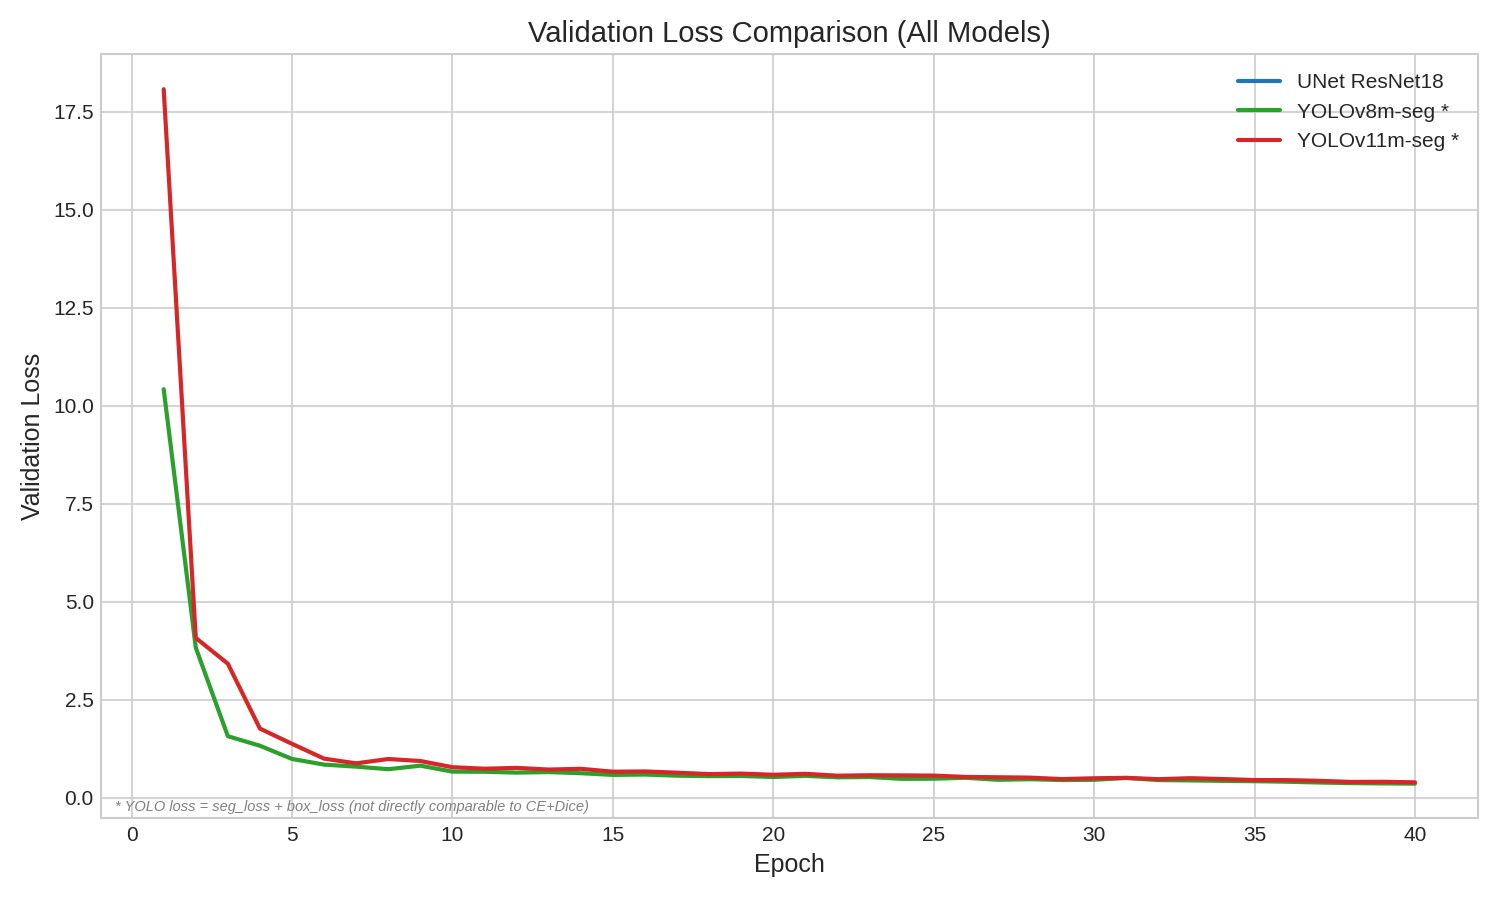
\includegraphics[width=0.75\textwidth]{plots_chignon/loss_curves.png}
    \caption{Courbes de perte (train/validation) --- Domaine Chignon.}
\end{figure}

\begin{figure}[H]
    \centering
    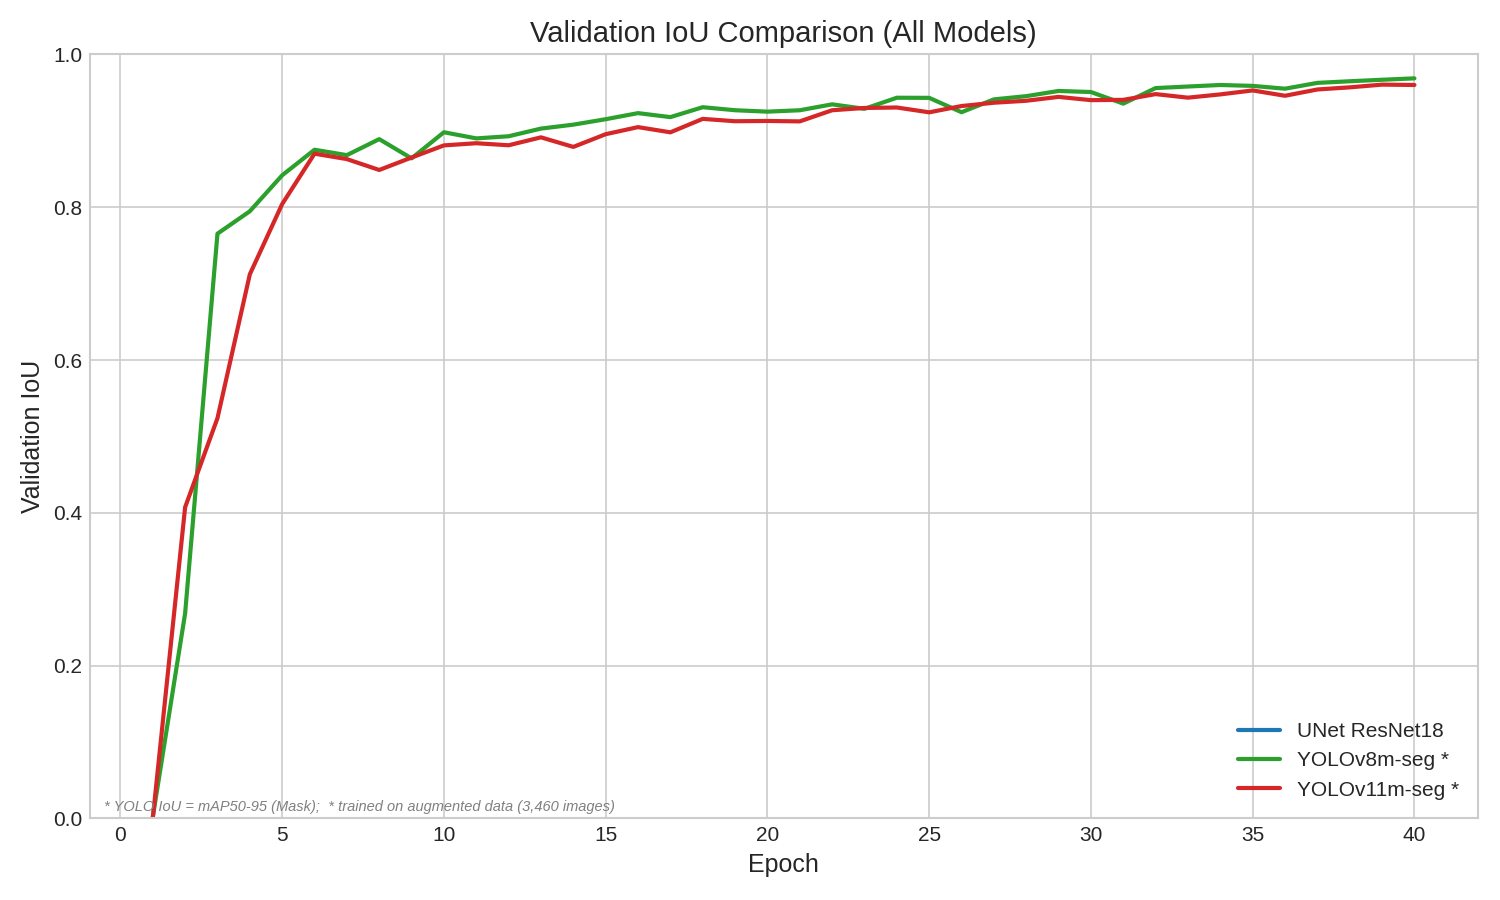
\includegraphics[width=0.75\textwidth]{plots_chignon/iou_curves.png}
    \caption{Courbes IoU (train/validation) --- Domaine Chignon par mod\`ele.}
\end{figure}

\begin{figure}[H]
    \centering
    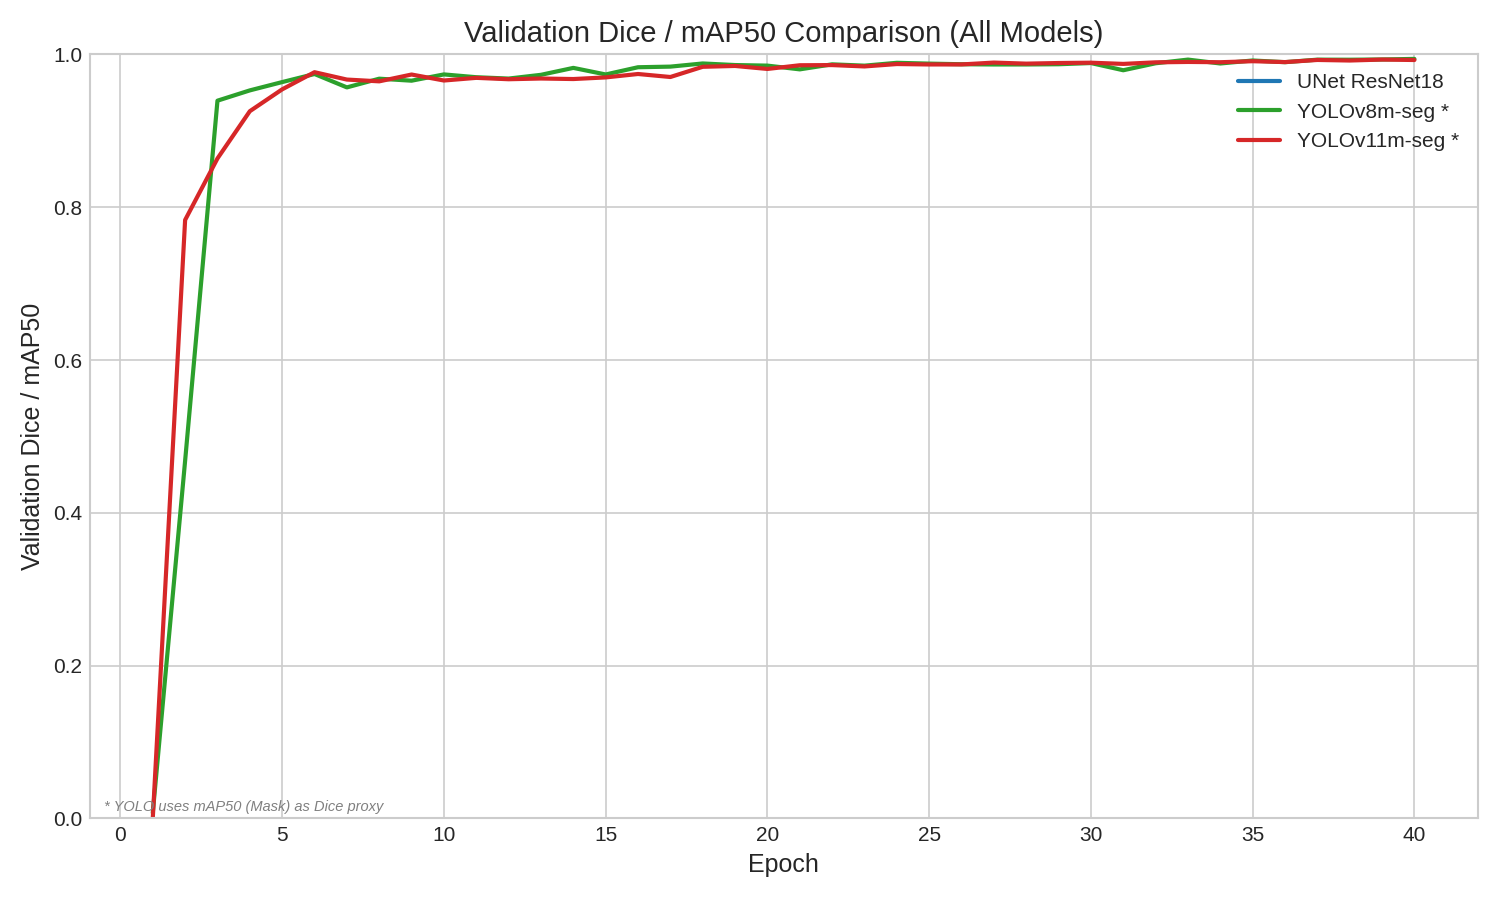
\includegraphics[width=0.75\textwidth]{plots_chignon/dice_curves.png}
    \caption{Courbes du coefficient Dice --- Domaine Chignon par mod\`ele.}
\end{figure}

\begin{figure}[H]
    \centering
    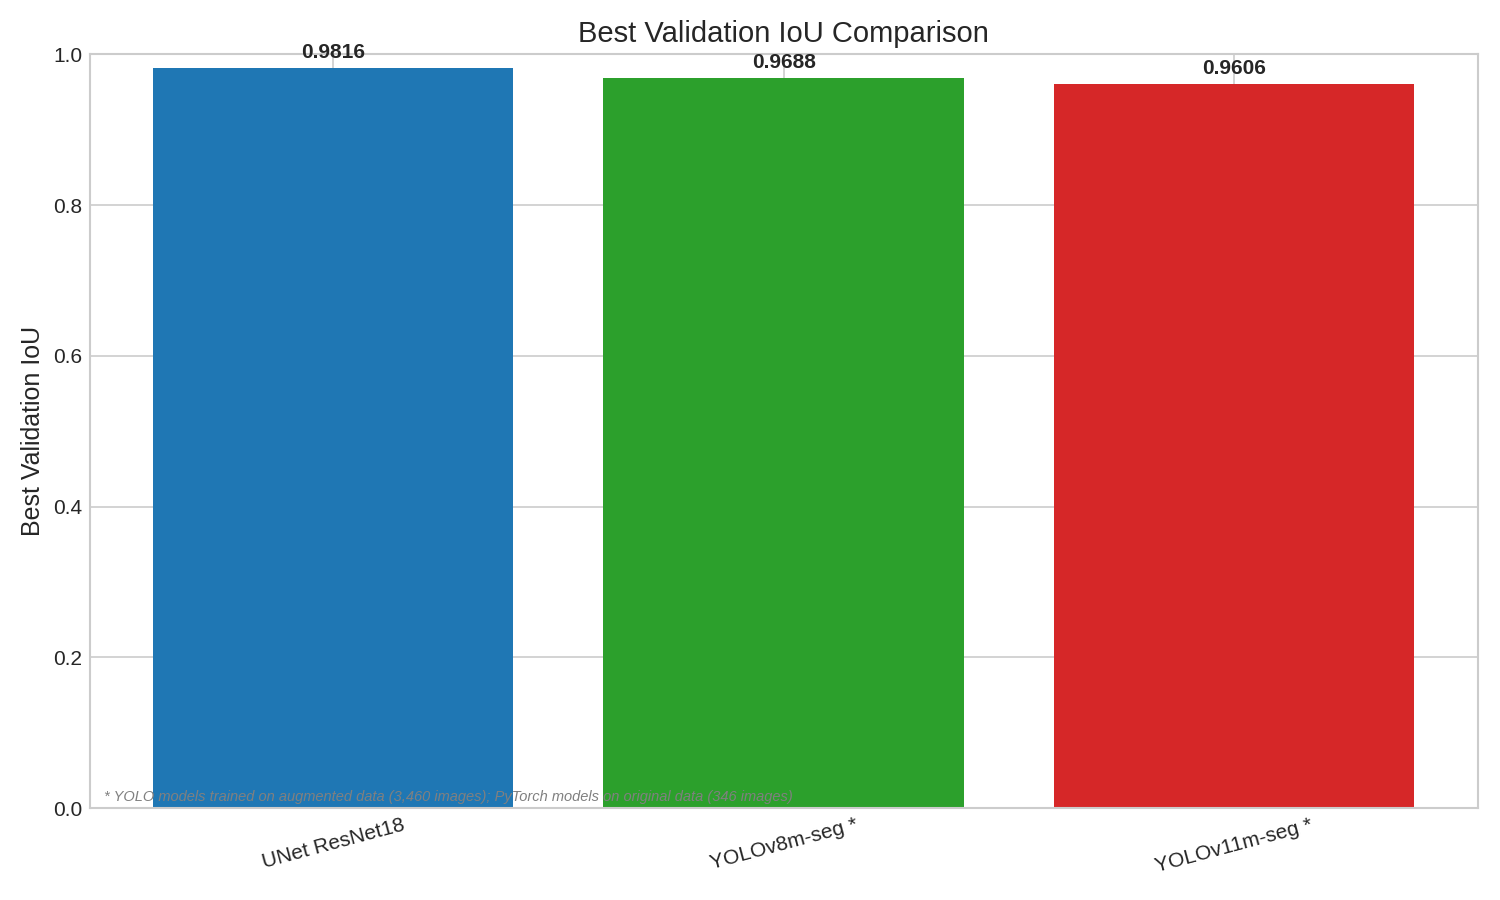
\includegraphics[width=0.70\textwidth]{plots_chignon/best_iou_comparison.png}
    \caption{Comparaison du meilleur IoU atteint par chaque mod\`ele --- Domaine Chignon.}
\end{figure}

\begin{figure}[H]
    \centering
    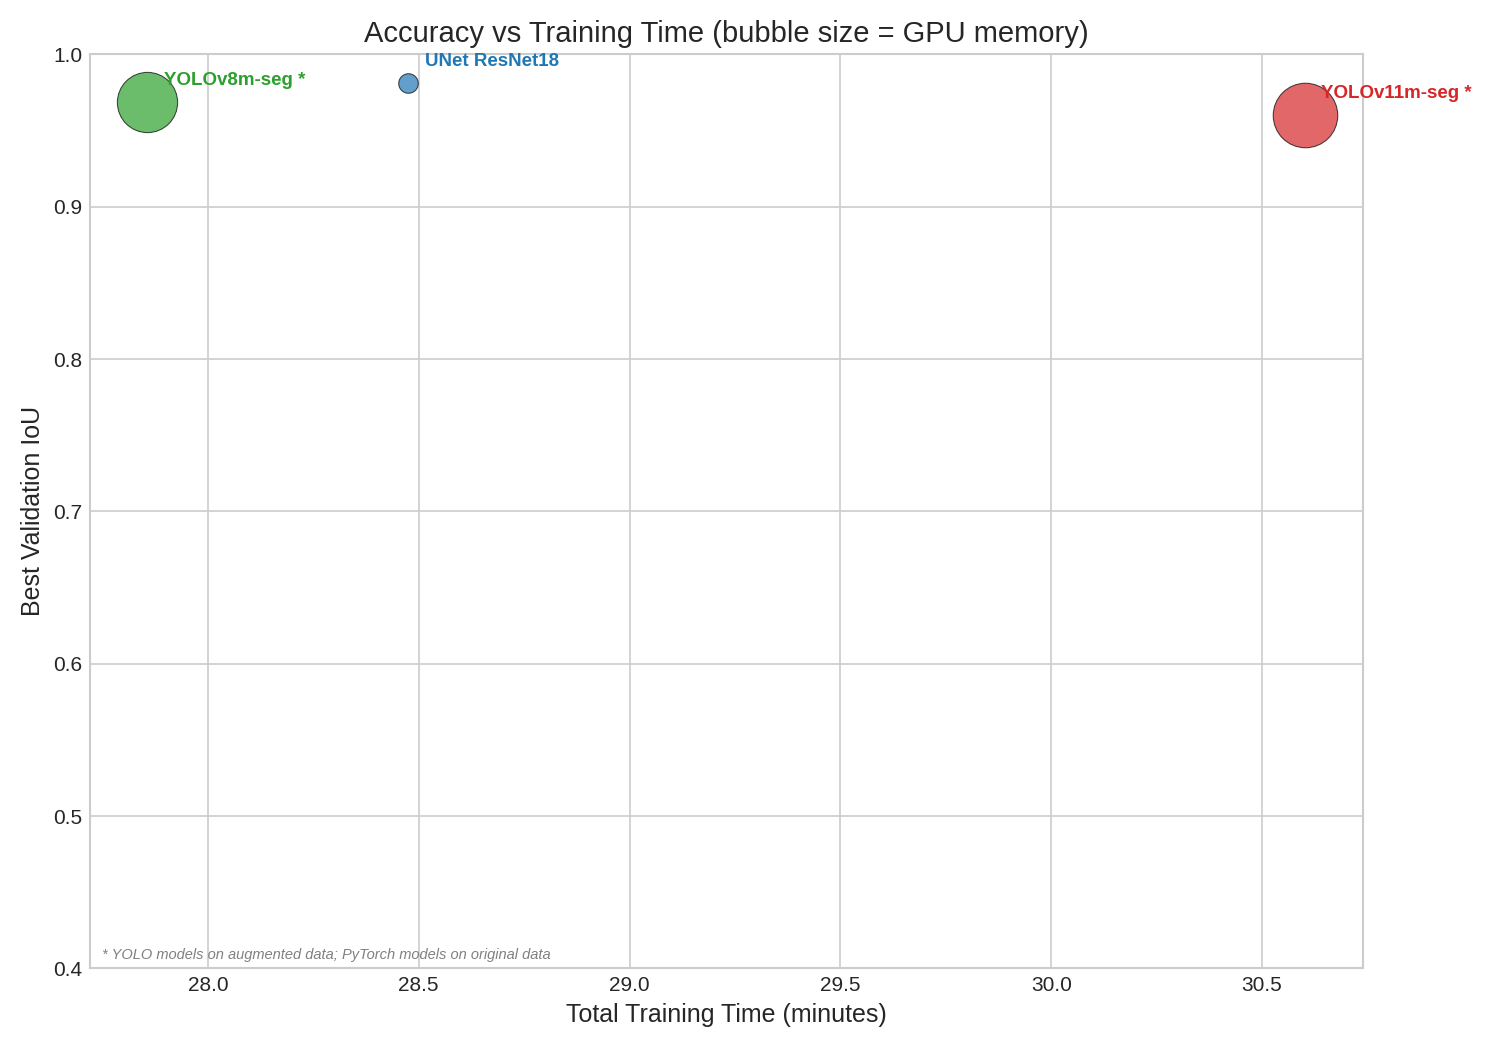
\includegraphics[width=0.70\textwidth]{plots_chignon/accuracy_vs_speed.png}
    \caption{Compromis pr\'ecision (IoU) vs. vitesse d'entra\^inement --- Domaine Chignon.}
\end{figure}

\begin{figure}[H]
    \centering
    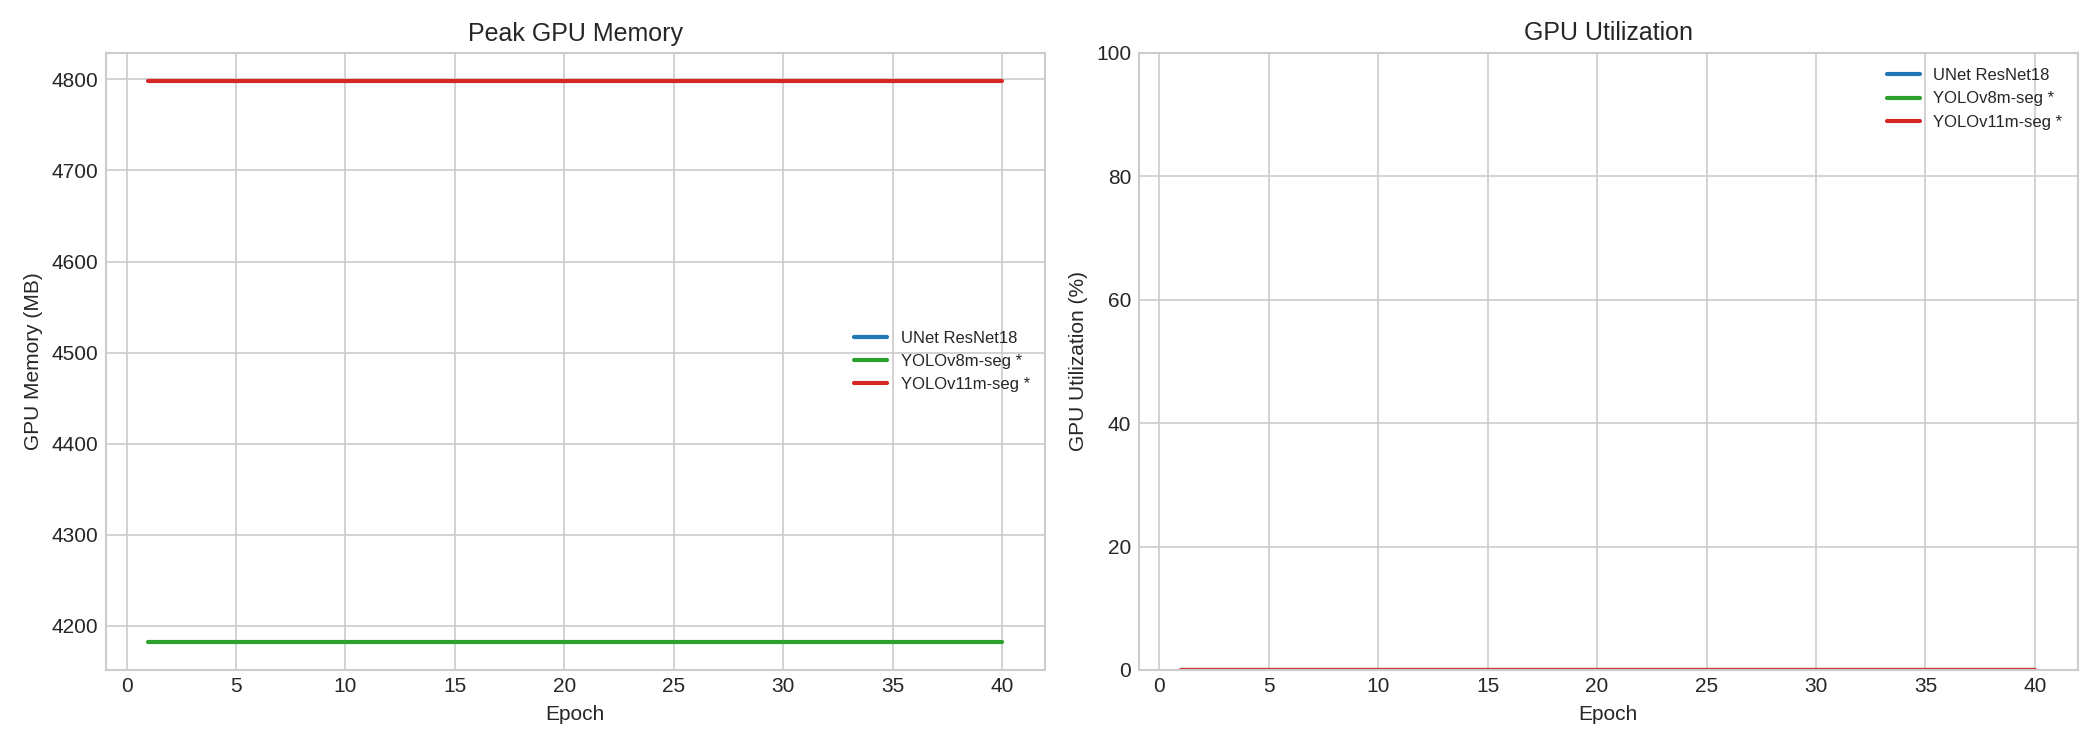
\includegraphics[width=0.75\textwidth]{plots_chignon/gpu_usage.png}
    \caption{Consommation m\'emoire GPU par mod\`ele --- Domaine Chignon.}
\end{figure}

\begin{figure}[H]
    \centering
    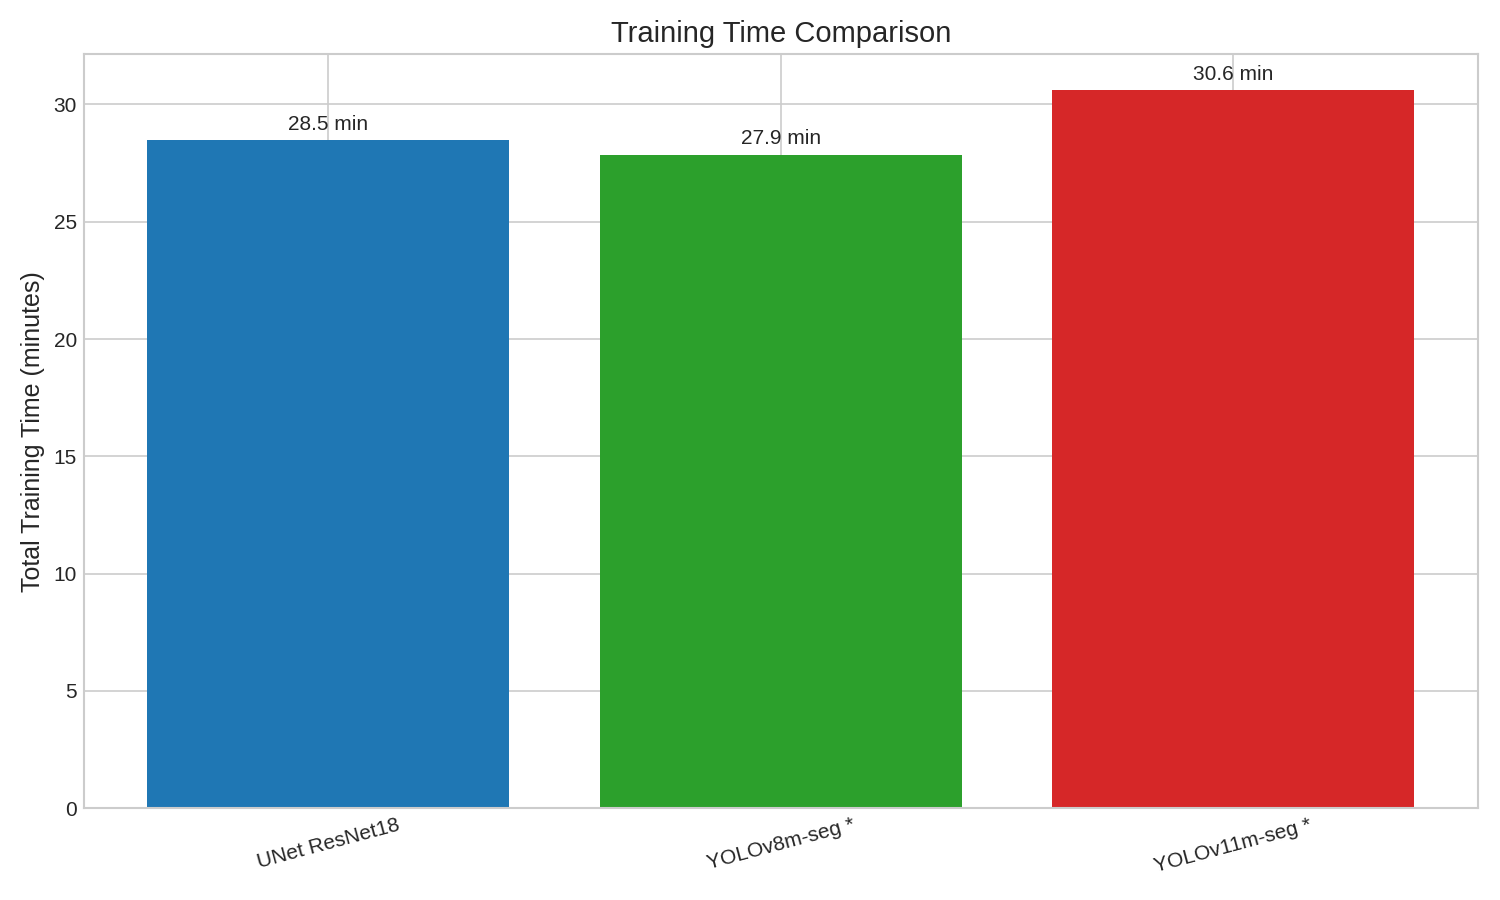
\includegraphics[width=0.70\textwidth]{plots_chignon/training_time.png}
    \caption{Temps d'entra\^inement total par mod\`ele --- Domaine Chignon.}
\end{figure}

\begin{figure}[H]
    \centering
    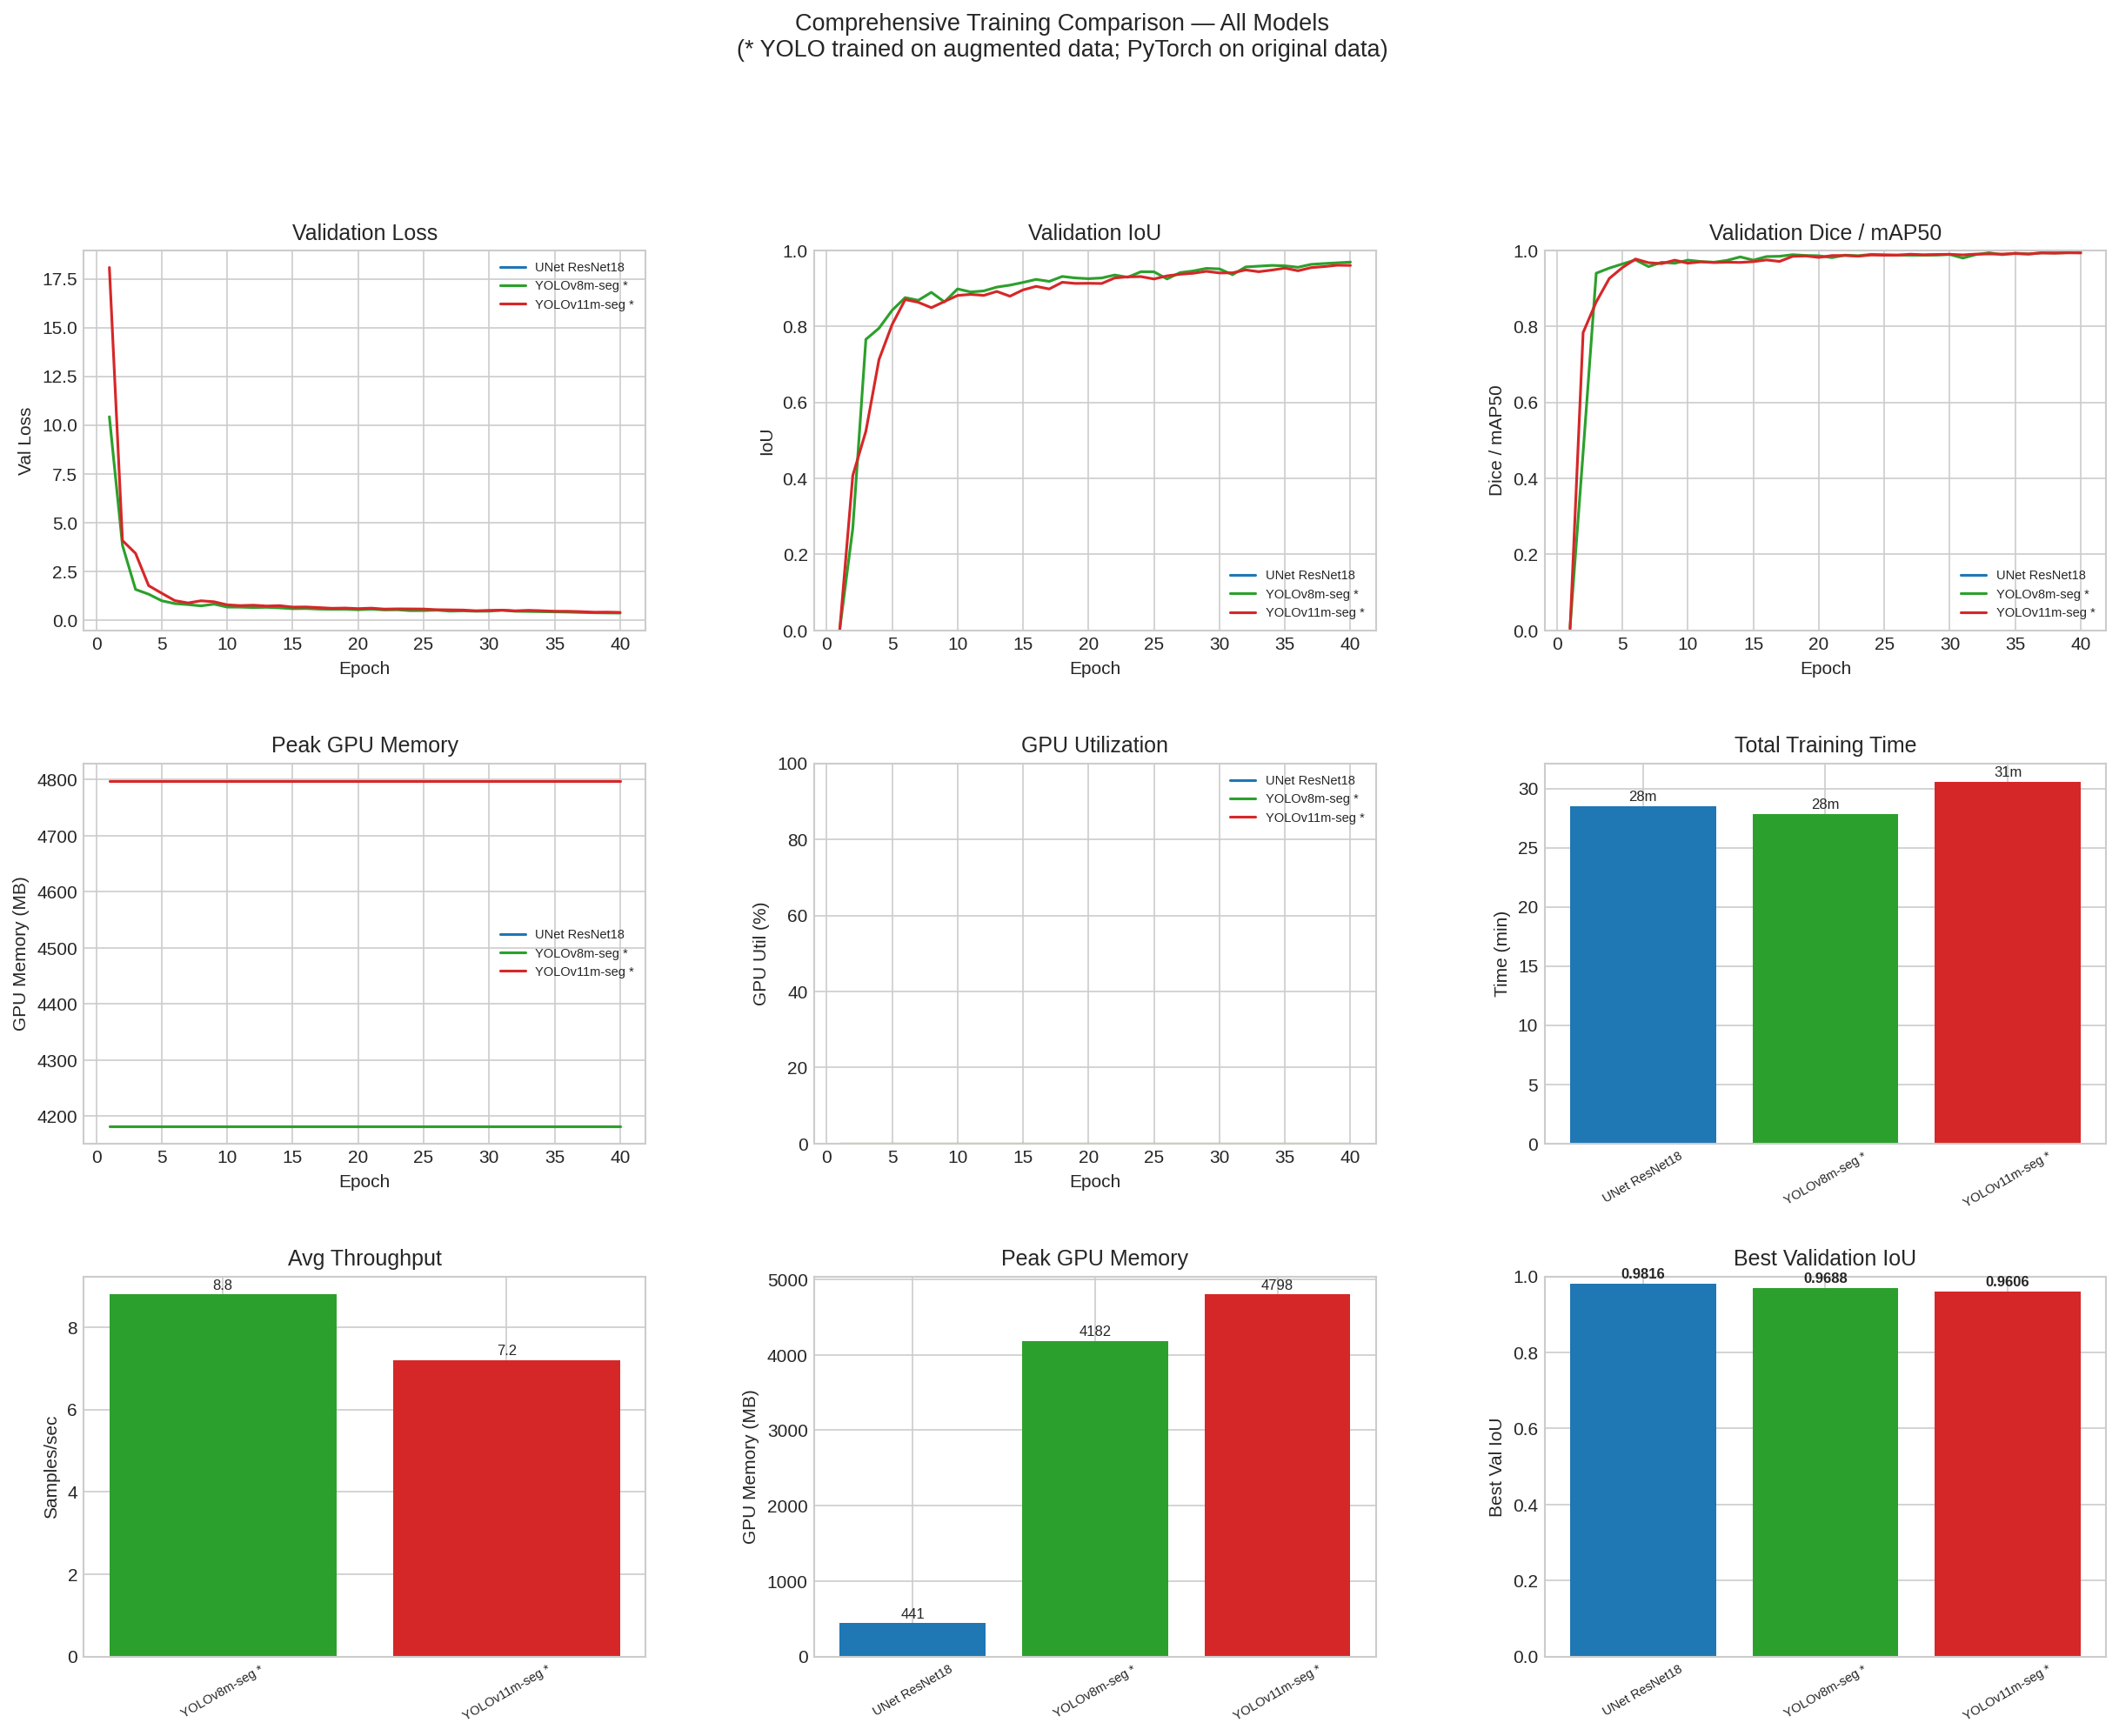
\includegraphics[width=0.75\textwidth]{plots_chignon/comprehensive_comparison.png}
    \caption{Tableau comparatif complet des mod\`eles --- Domaine Chignon.}
\end{figure}

\begin{figure}[H]
    \centering
    \begin{subfigure}[b]{0.48\textwidth}
        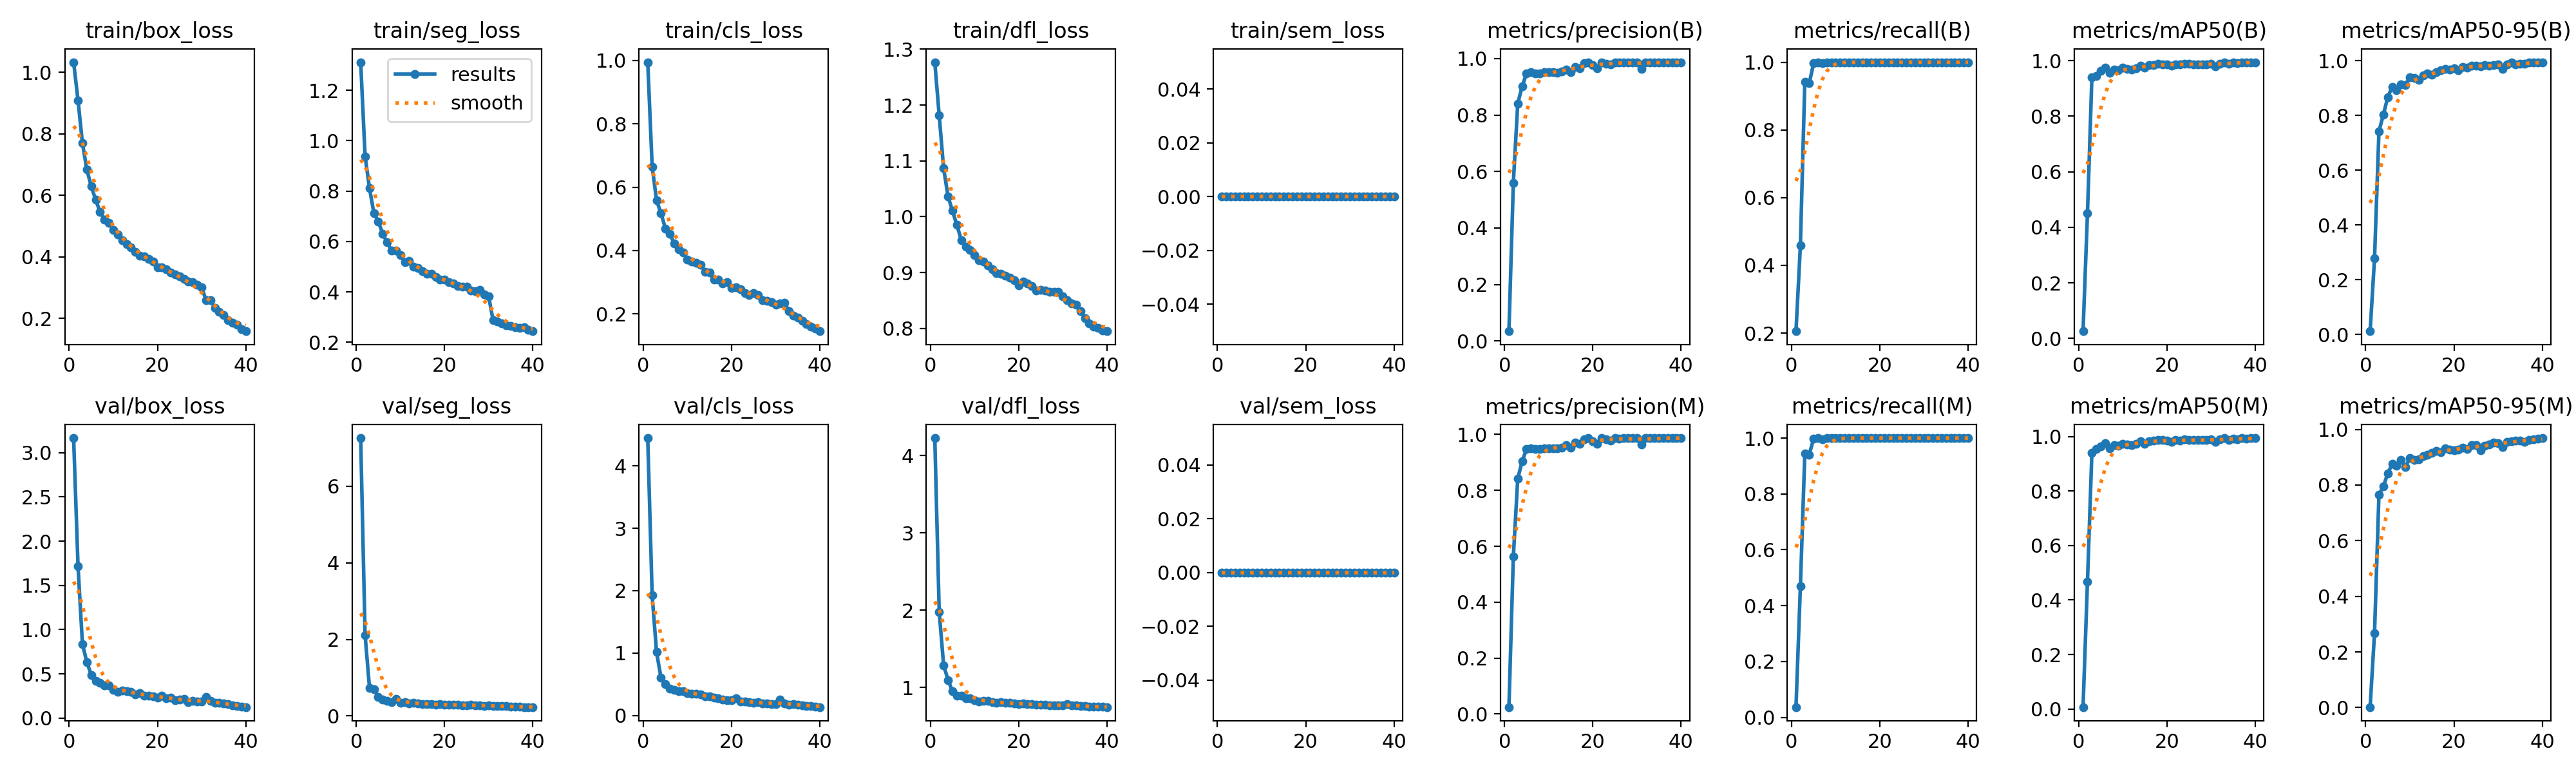
\includegraphics[width=\textwidth]{plots_chignon/yolov8m_results.png}
        \caption{YOLOv8m Seg}
    \end{subfigure}
    \hfill
    \begin{subfigure}[b]{0.48\textwidth}
        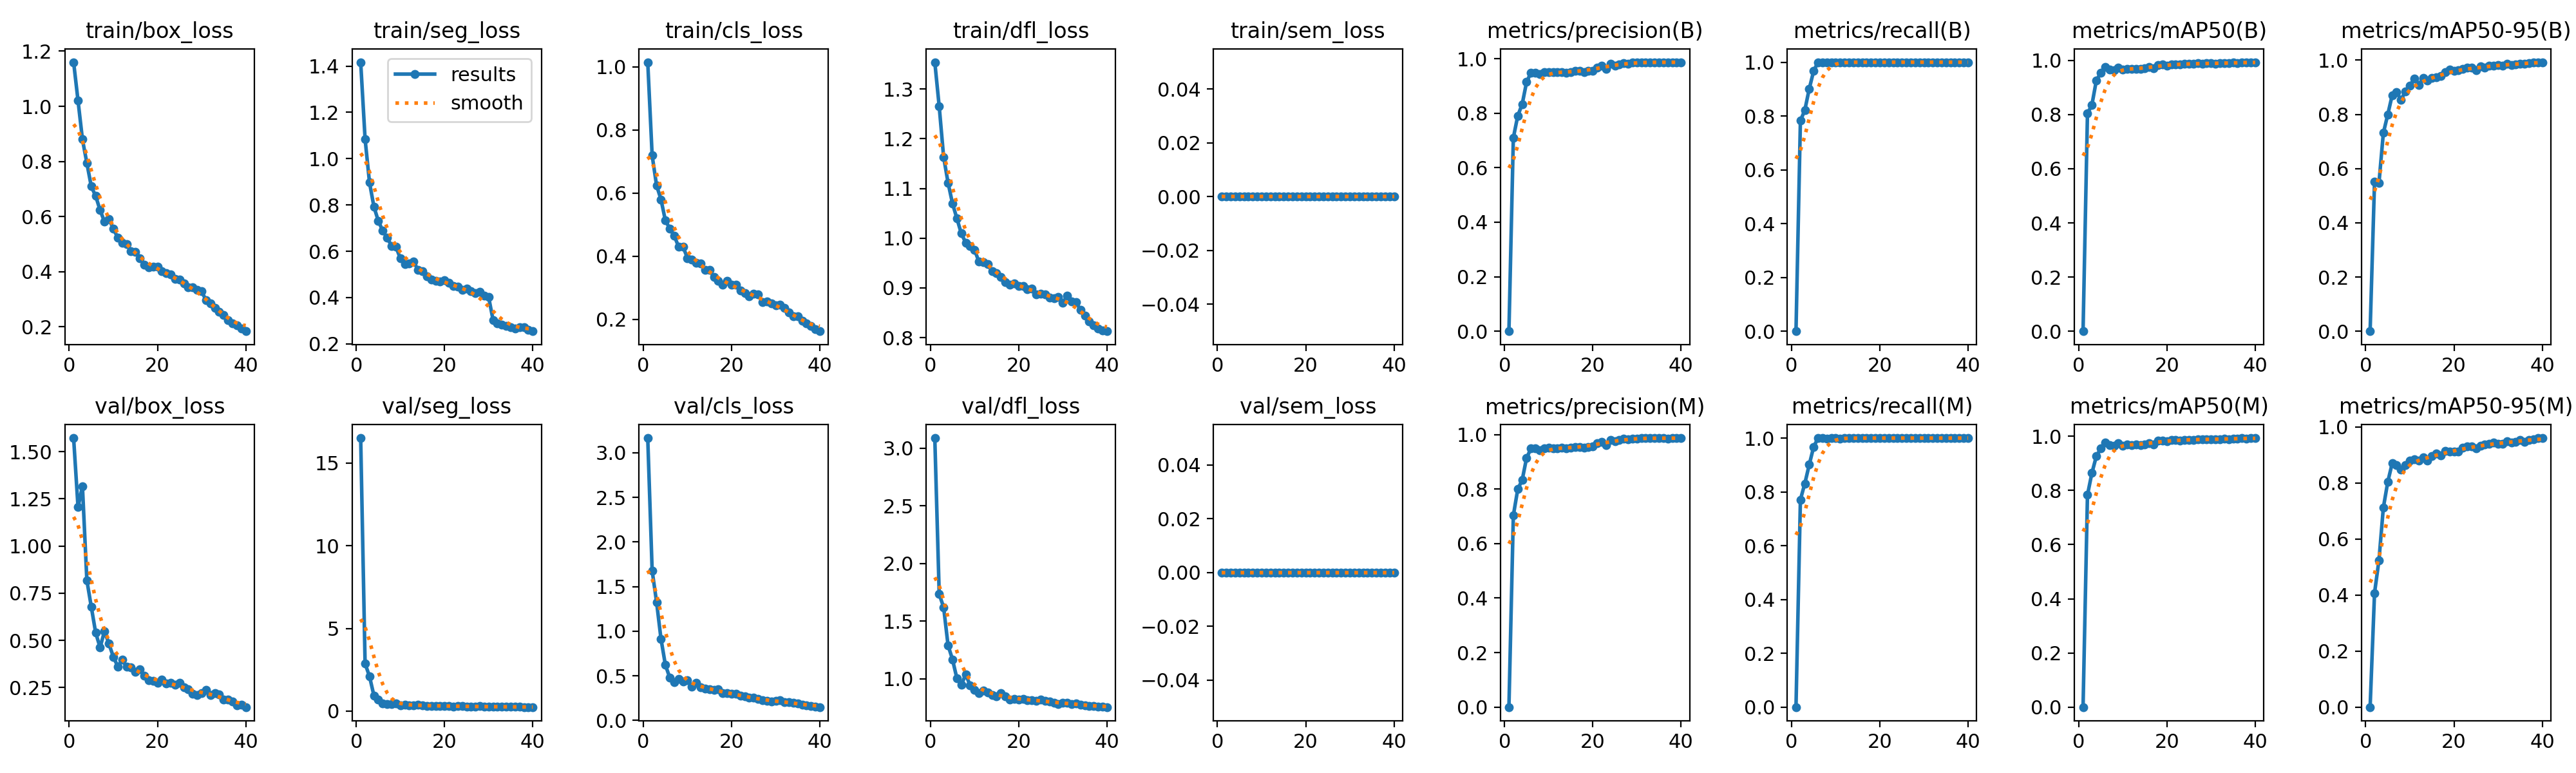
\includegraphics[width=\textwidth]{plots_chignon/yolov11m_results.png}
        \caption{YOLOv11m Seg}
    \end{subfigure}
    \caption{Tableaux de bord YOLO Ultralytics --- Domaine Chignon.}
\end{figure}

\begin{figure}[H]
    \centering
    \begin{subfigure}[b]{0.48\textwidth}
        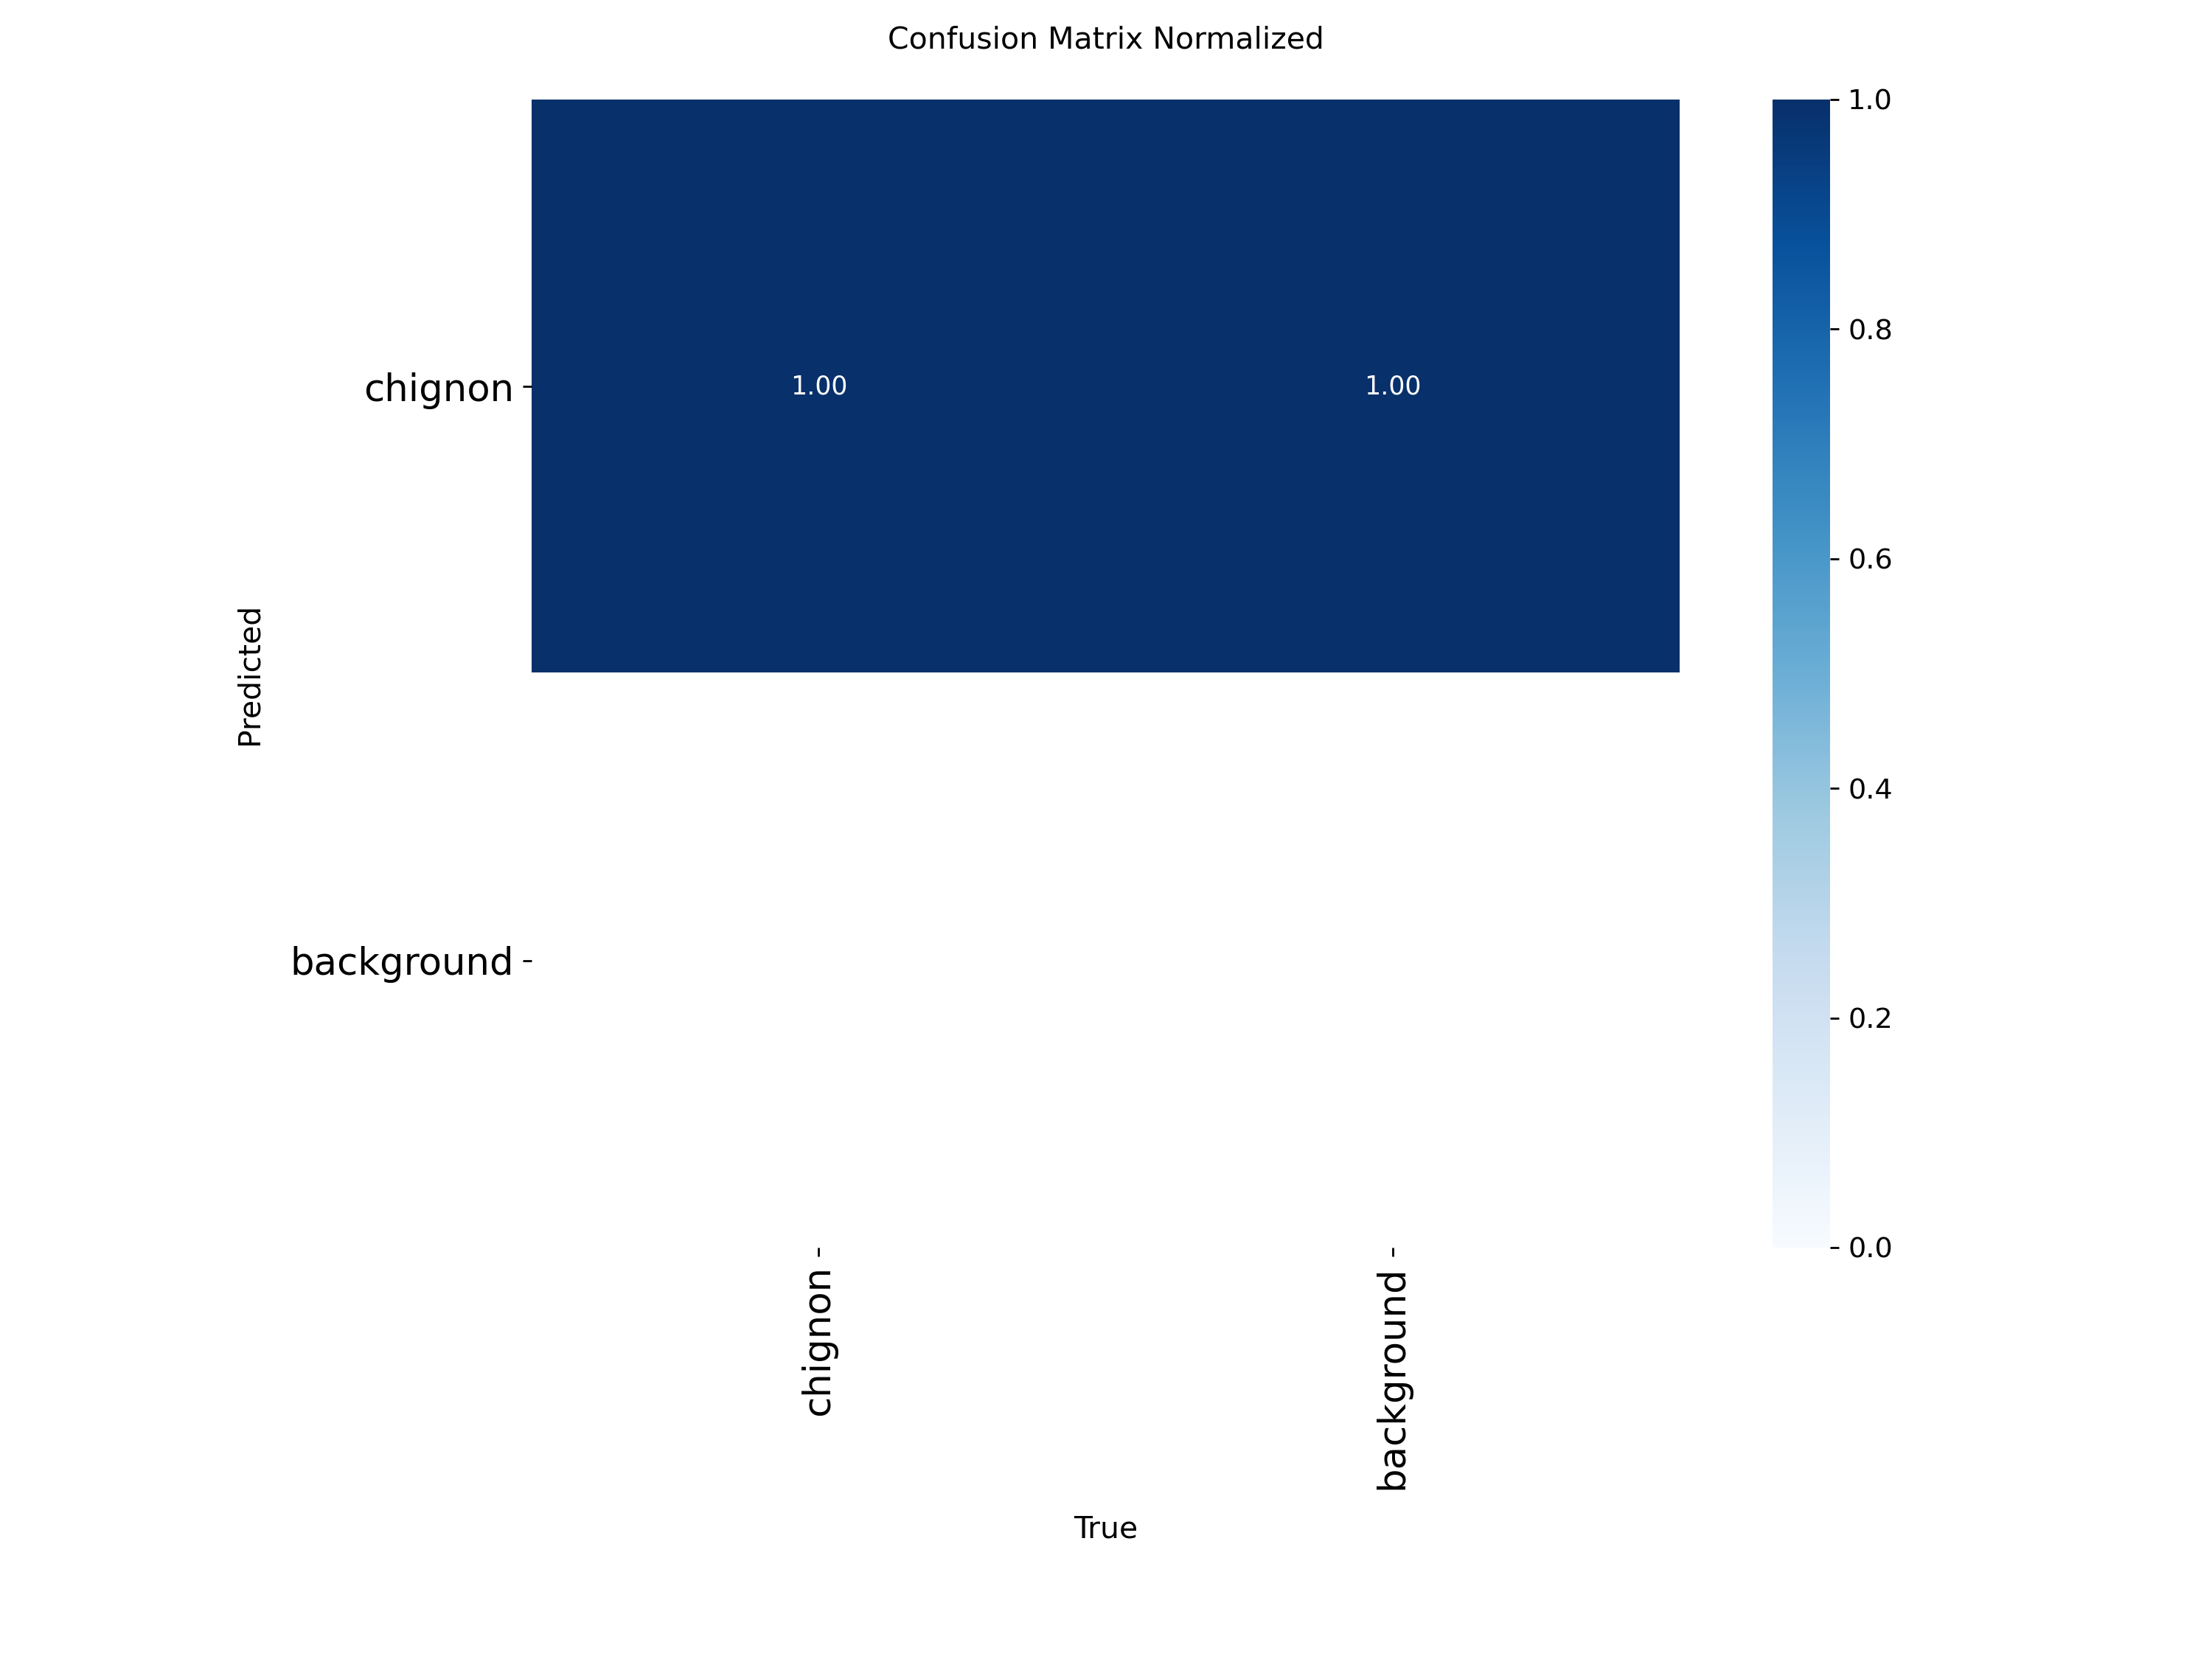
\includegraphics[width=\textwidth]{plots_chignon/yolov8m_confusion.png}
        \caption{YOLOv8m Seg}
    \end{subfigure}
    \hfill
    \begin{subfigure}[b]{0.48\textwidth}
        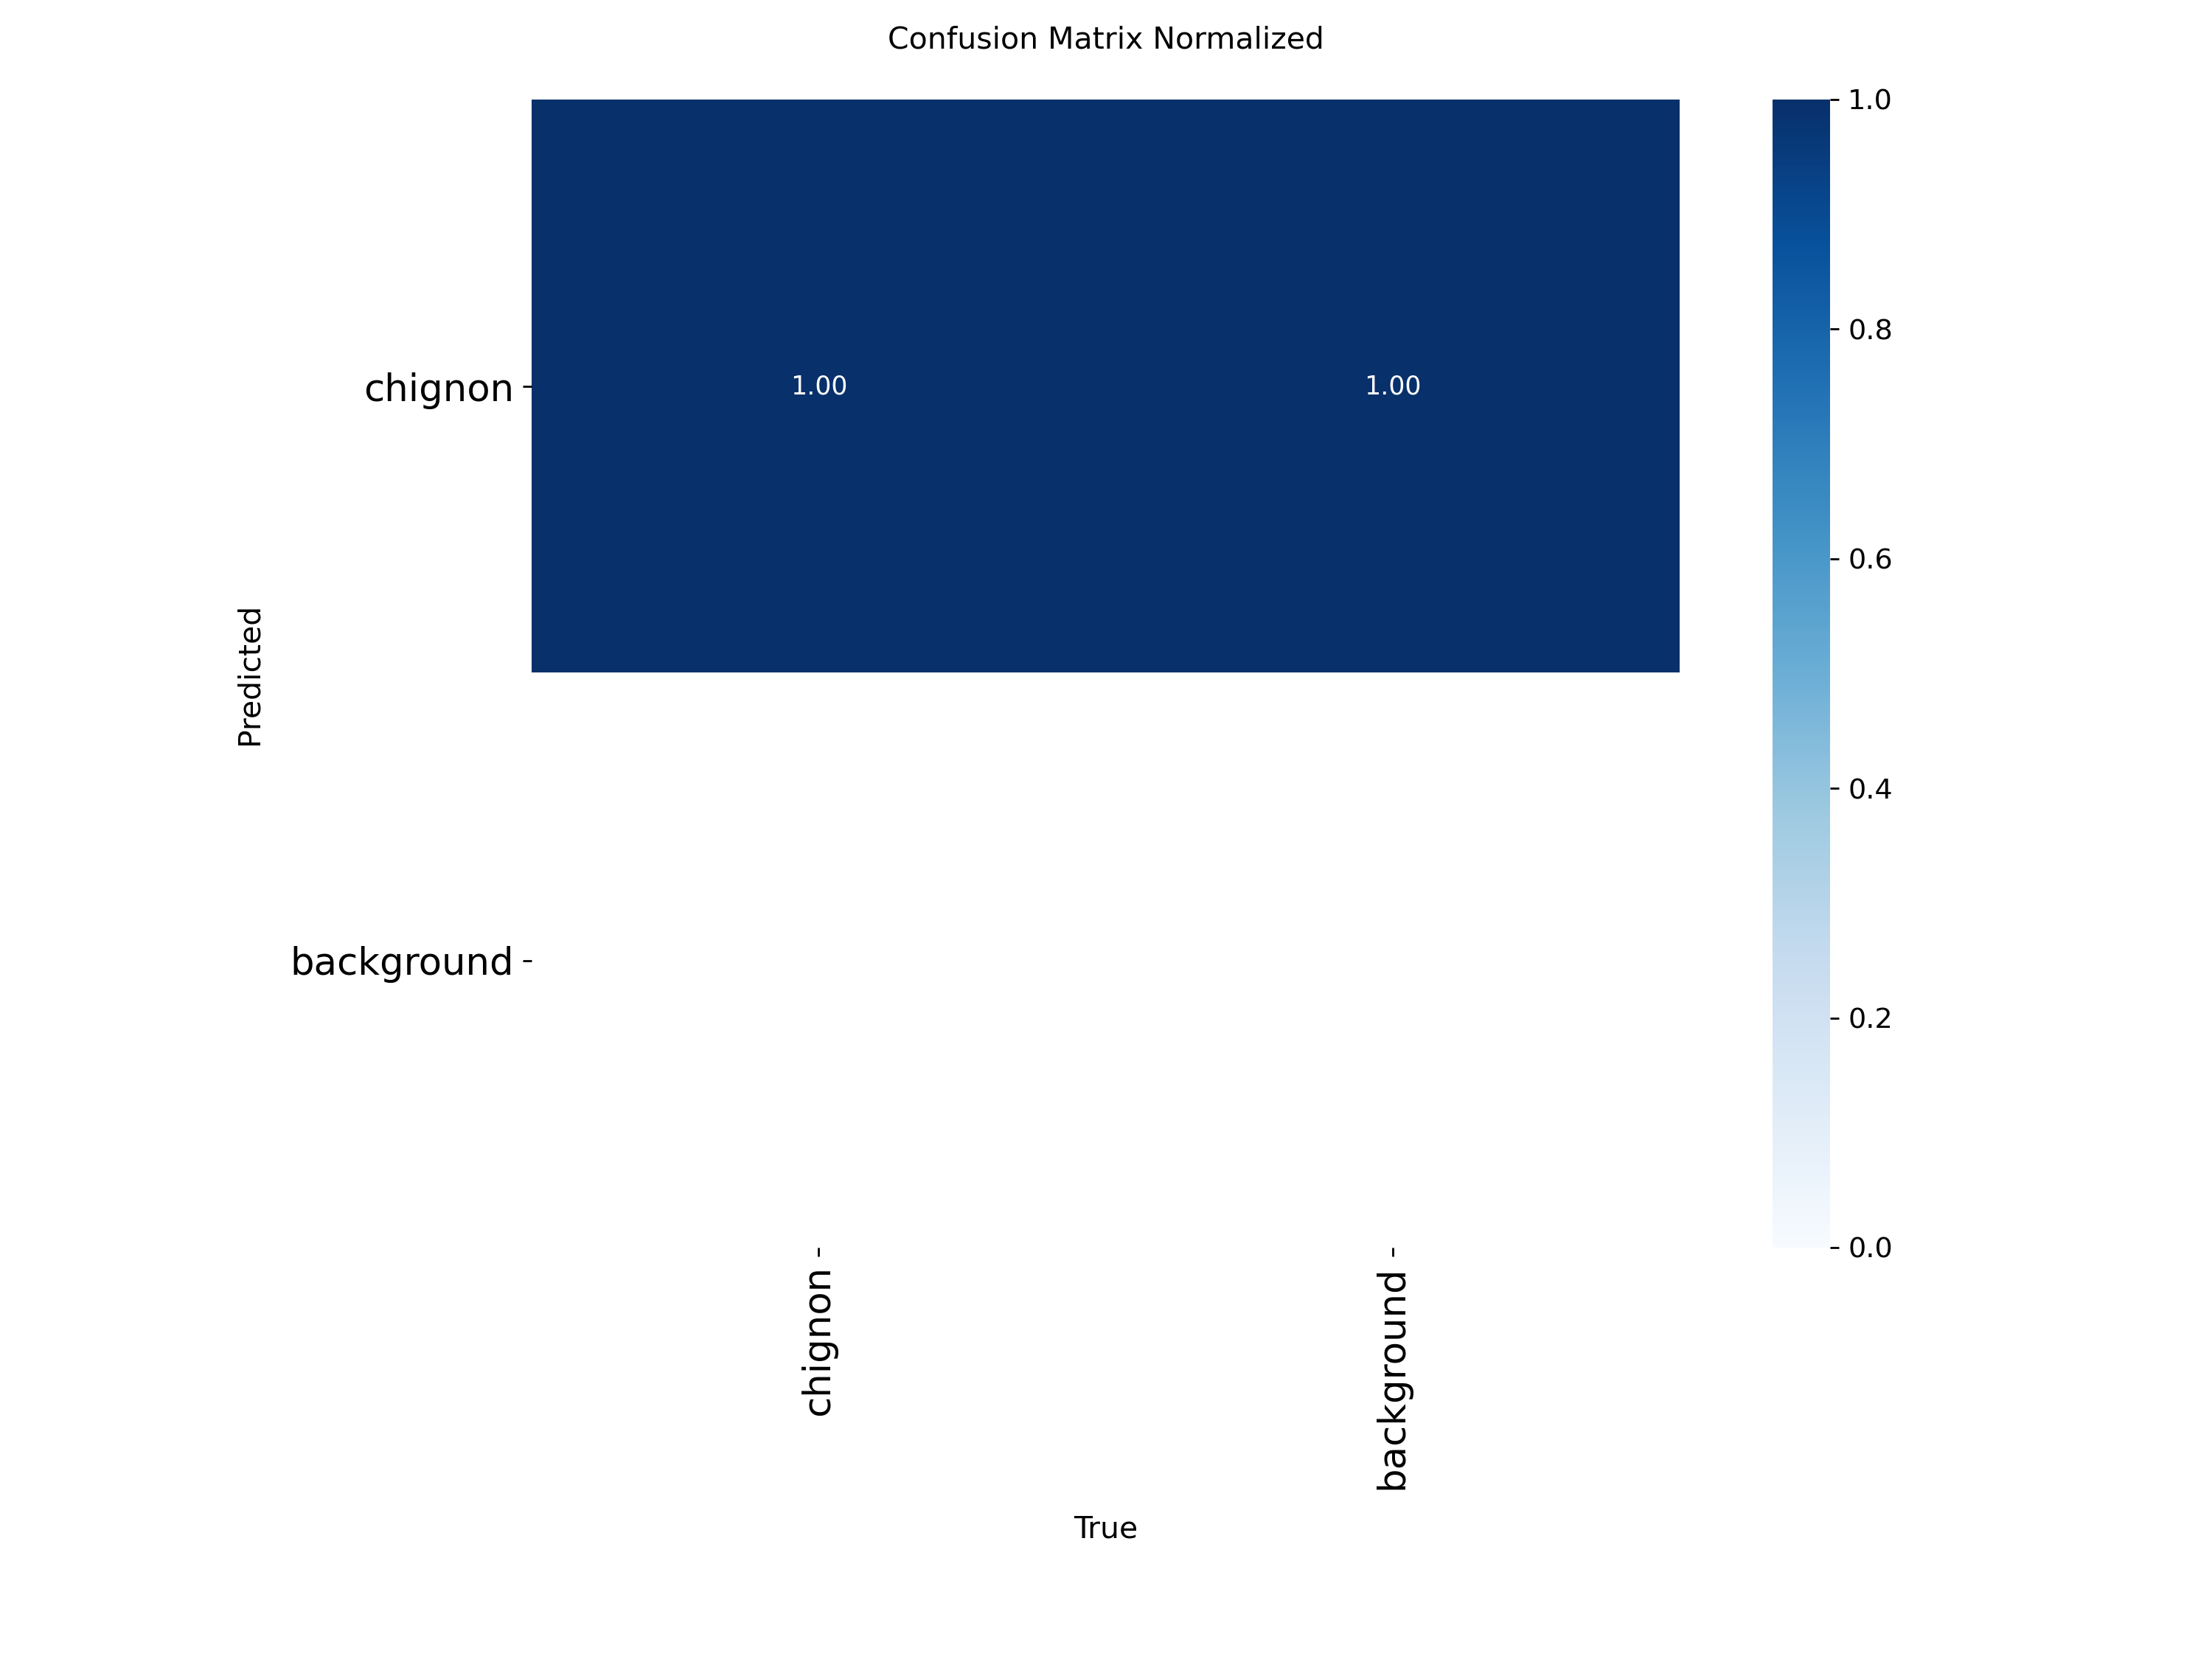
\includegraphics[width=\textwidth]{plots_chignon/yolov11m_confusion.png}
        \caption{YOLOv11m Seg}
    \end{subfigure}
    \caption{Matrices de confusion normalis\'ees YOLO --- Domaine Chignon.}
\end{figure}

% -----------------------------------------------------------------------
\section{Domaine Files (C\^ables)}

\subsection{R\'esultats comparatifs et analyse des \'echecs YOLO}

\begin{table}[H]
\centering
\begin{tabular}{lcccc}
\toprule
\textbf{Mod\`ele} & \textbf{Val IoU} & \textbf{\'Epoque opt.} & \textbf{GPU Peak (MB)} & \textbf{Temps (s)} \\
\midrule
UNet ResNet18~\cite{ronneberger2015unet,he2016resnet}    & \textbf{0.9197}  & 30  & 440.9  & 1\,000 \\
YOLOv8m Seg~\cite{jocher2023yolov8}      & N/A              & ---   & 3\,964 & 810 \\
YOLOv11m Seg     & N/A              & ---   & 4\,736 & 898 \\
\bottomrule
\end{tabular}
\caption{R\'esultats d'entra\^inement --- Domaine Files (2 classes). Les mod\`eles YOLO n'ont pas converg\'e pour ce domaine.}
\label{tab:files_results}
\end{table}

La non-convergence des mod\`eles YOLO sur le domaine c\^ables s'explique par la nature morphologique des objets~: les c\^ables sont des structures fines et allong\'ees, dont les \textit{bounding boxes} sont de rapport d'aspect extr\^eme. Les architectures YOLO, optimis\'ees pour des objets compacts, peinent \`a mod\'eliser des instances lin\'eaires. En revanche, UNet~\cite{ronneberger2015unet}, avec sa segmentation pixel-\`a-pixel et ses connexions de saut pr\'eservant les d\'etails fins, g\`ere naturellement ces configurations.

\subsection{Courbes d'entra\^inement --- Files}

\begin{figure}[H]
    \centering
    
\includegraphics[width=0.75\textwidth]{plots_files/loss_curves.png}
    \caption{Courbes de perte (train/validation) --- Domaine Files.}
\end{figure}

\begin{figure}[H]
    \centering
    
\includegraphics[width=0.75\textwidth]{plots_files/iou_curves.png}
    \caption{Courbes IoU (train/validation) --- Domaine Files par mod\`ele.}
\end{figure}

\begin{figure}[H]
    \centering
    
\includegraphics[width=0.75\textwidth]{plots_files/dice_curves.png}
    \caption{Courbes du coefficient Dice --- Domaine Files par mod\`ele.}
\end{figure}

\begin{figure}[H]
    \centering
    
\includegraphics[width=0.70\textwidth]{plots_files/best_iou_comparison.png}
    \caption{Comparaison du meilleur IoU atteint par chaque mod\`ele --- Domaine Files.}
\end{figure}

\begin{figure}[H]
    \centering
    
\includegraphics[width=0.70\textwidth]{plots_files/accuracy_vs_speed.png}
    \caption{Compromis pr\'ecision (IoU) vs. vitesse d'entra\^inement --- Domaine Files.}
\end{figure}

\begin{figure}[H]
    \centering
    
\includegraphics[width=0.75\textwidth]{plots_files/gpu_usage.png}
    \caption{Consommation m\'emoire GPU par mod\`ele --- Domaine Files.}
\end{figure}

\begin{figure}[H]
    \centering
    
\includegraphics[width=0.70\textwidth]{plots_files/training_time.png}
    \caption{Temps d'entra\^inement total par mod\`ele --- Domaine Files.}
\end{figure}

\begin{figure}[H]
    \centering
    
\includegraphics[width=0.75\textwidth]{plots_files/comprehensive_comparison.png}
    \caption{Tableau comparatif complet des mod\`eles --- Domaine Files.}
\end{figure}

\begin{figure}[H]
    \centering
    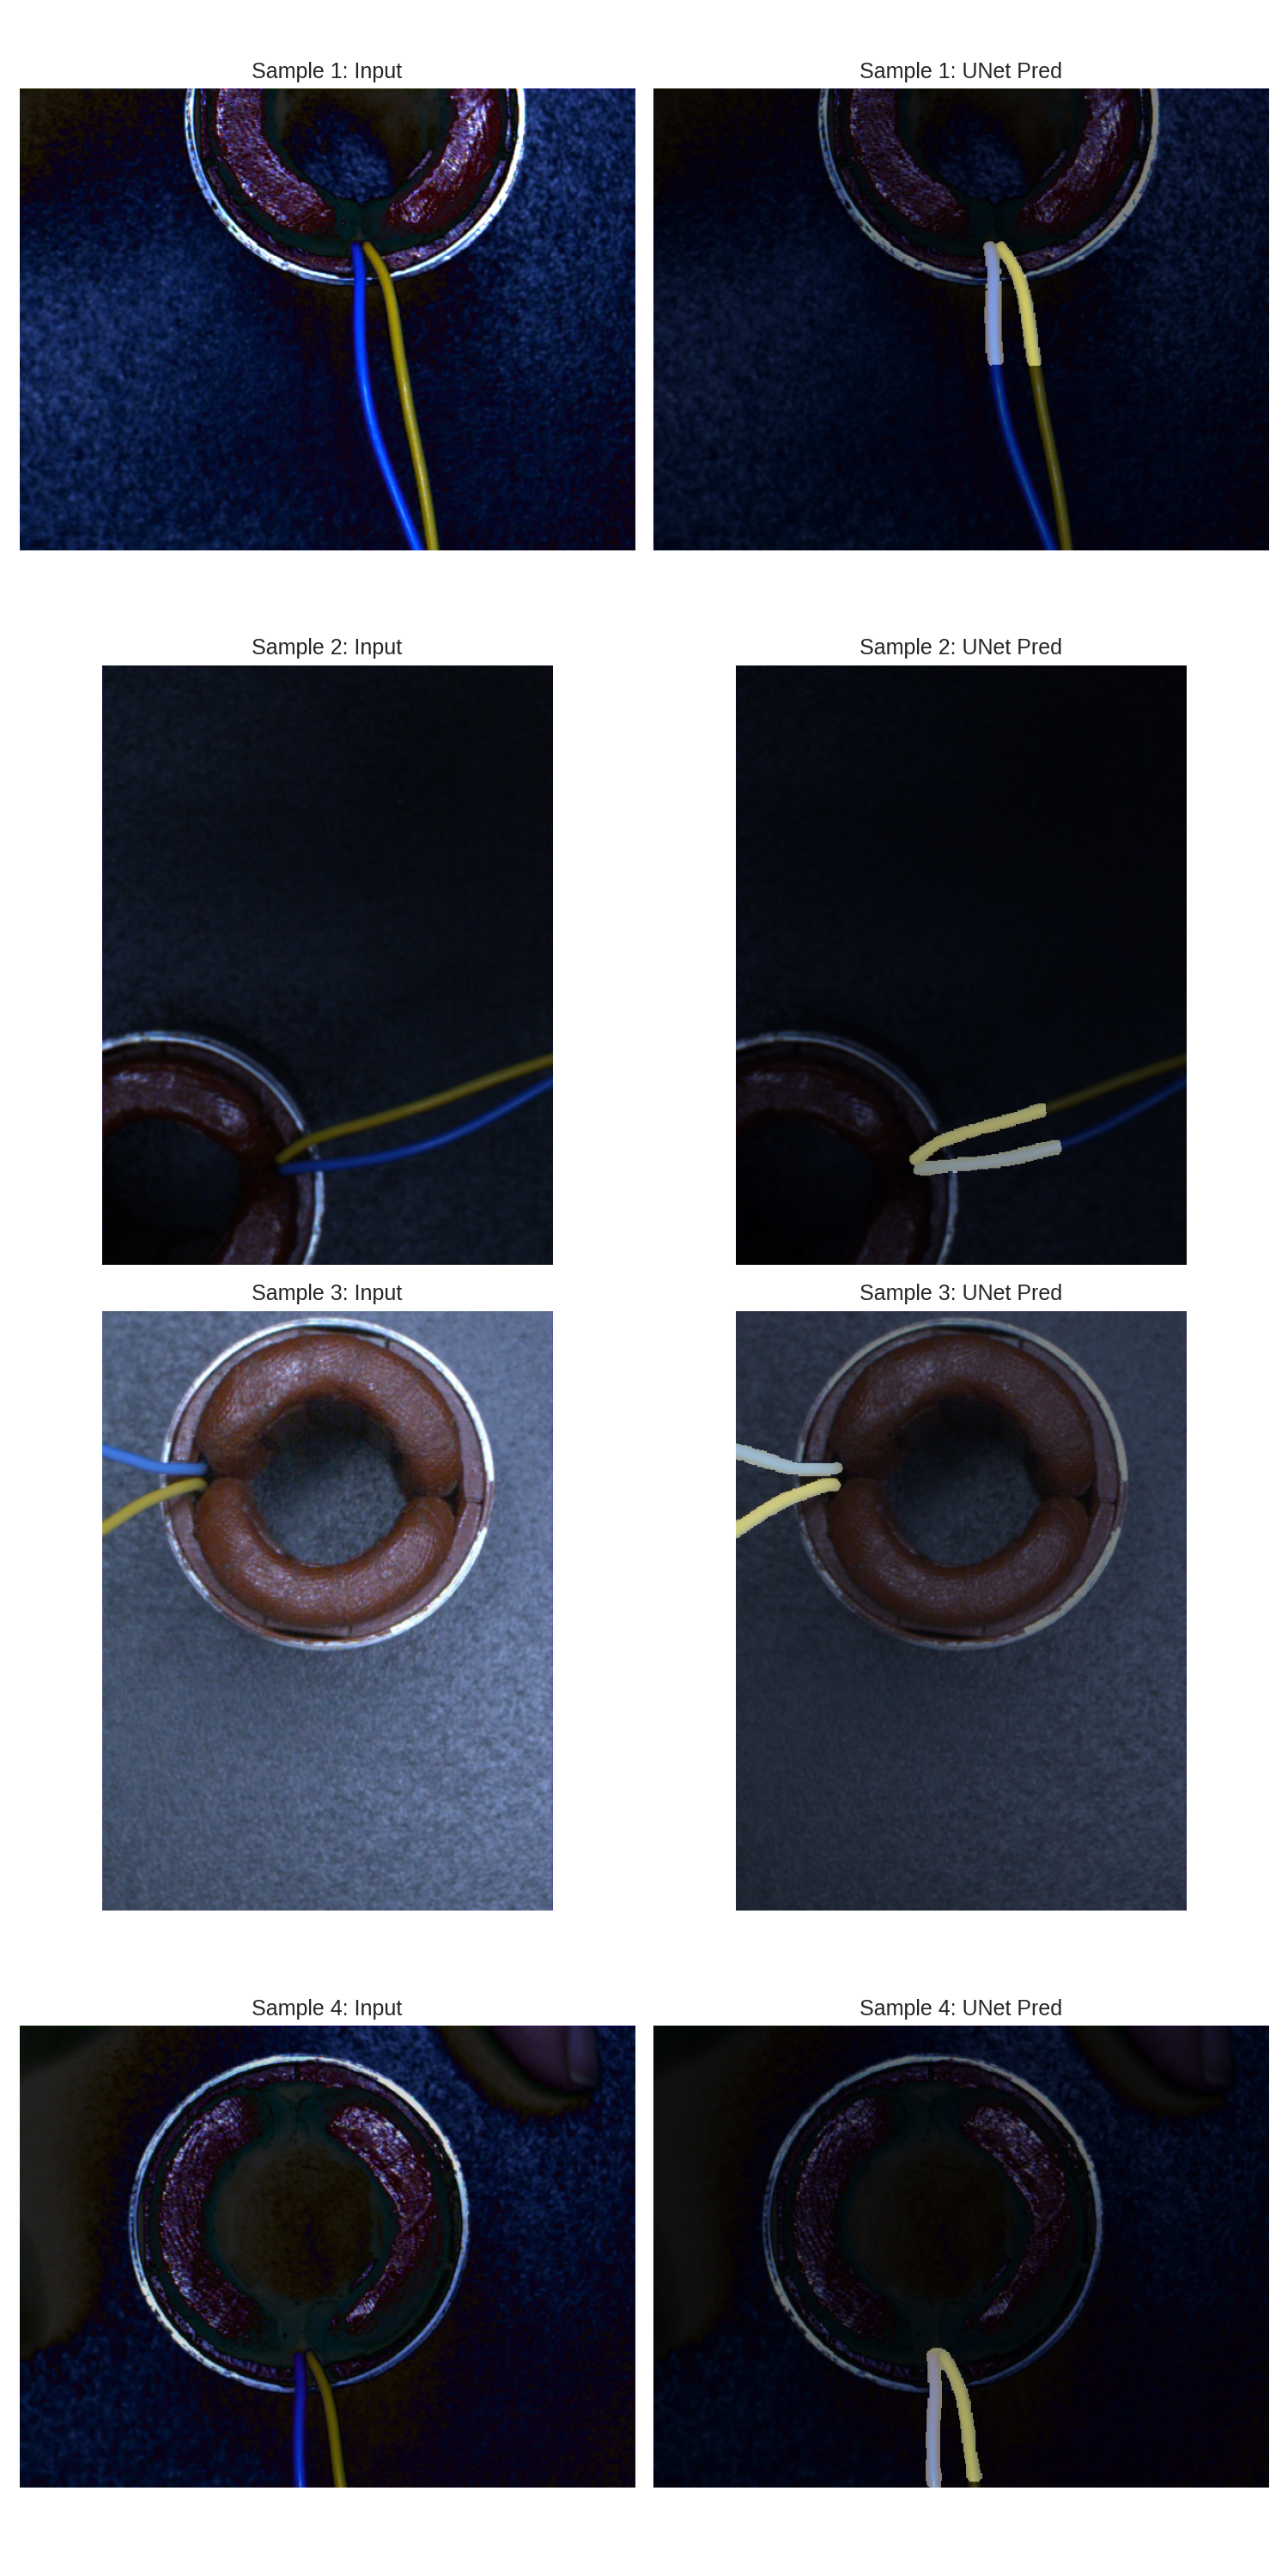
\includegraphics[width=0.75\textwidth]{plots_files/test_set_visual_verification.png}
    \caption{V\'erification visuelle sur le jeu de test --- Domaine Files.}
\end{figure}

\begin{figure}[H]
    \centering
    \begin{subfigure}[b]{0.48\textwidth}
        
\includegraphics[width=\textwidth]{plots_files/yolov8m_results.png}
        \caption{YOLOv8m Seg}
    \end{subfigure}
    \hfill
    \begin{subfigure}[b]{0.48\textwidth}
        
\includegraphics[width=\textwidth]{plots_files/yolov11m_results.png}
        \caption{YOLOv11m Seg}
    \end{subfigure}
    \caption{Tableaux de bord YOLO Ultralytics --- Domaine Files (pas de convergence observ\'ee).}
\end{figure}

\begin{figure}[H]
    \centering
    \begin{subfigure}[b]{0.48\textwidth}
        
\includegraphics[width=\textwidth]{plots_files/yolov8m_confusion.png}
        \caption{YOLOv8m Seg}
    \end{subfigure}
    \hfill
    \begin{subfigure}[b]{0.48\textwidth}
        
\includegraphics[width=\textwidth]{plots_files/yolov11m_confusion.png}
        \caption{YOLOv11m Seg}
    \end{subfigure}
    \caption{Matrices de confusion normalis\'ees YOLO --- Domaine Files.}
\end{figure}


% ==========================================================================
\chapter{Pipeline de D\'etection}
% ==========================================================================

\begin{figure}[H]
    \centering
    
\includegraphics[width=0.50\textwidth]{detection_pipeline.png}
    \caption{Pipeline de d\'etection complet --- De l'acquisition d'image (WebRTC, upload, cam\'era industrielle) au tableau de bord, en passant par le routage de domaine, l'inf\'erence, le post-traitement et le moteur de mesure g\'eom\'etrique.}
    \label{fig:detection_pipeline}
\end{figure}

\section{Sources d'entr\'ee}

Le syst\`eme accepte trois sources d'entr\'ee compl\'ementaires~:
\begin{enumerate}
    \item \textbf{WebRTC} --- Flux cam\'era \textit{live} depuis le navigateur~: connexion directe sans latence r\'eseau significative, id\'eale pour l'inspection en temps r\'eel \`a la cha\^ine de production.
    \item \textbf{Upload d'image} --- Image fixe envoy\'ee via l'API REST~: adapt\'e \`a l'inspection diff\'er\'ee ou \`a l'int\'egration dans des syst\`emes existants.
    \item \textbf{Cam\'era MindVision} --- Cam\'era industrielle via SDK propri\'etaire~: r\'esolution et qualit\'e d'image sup\'erieures, adapt\'e aux exigences de mesure pr\'ecise.
\end{enumerate}

% -----------------------------------------------------------------------
\section{Pipeline de d\'etection --- Stator}

\begin{figure}[H]
    \centering
    
\includegraphics[width=0.50\textwidth]{stator_detection_pipeline.png}
    \caption{Pipeline de d\'etection d\'etaill\'e pour le domaine Stator, incluant la s\'election du mod\`ele, le post-traitement sp\'ecifique (filtre Top-N, correction heuristique spatiale, ByteTrack, Guided Filter), et le moteur de mesure g\'eom\'etrique \`a quatre m\'ethodes de calibration.}
    \label{fig:stator_detect}
\end{figure}

\subsection{D\'ecouverte automatique des mod\`eles}

Le syst\`eme scanne automatiquement les r\'epertoires de sortie pour d\'ecouvrir les mod\`eles disponibles. Les formats sont prioris\'es dans l'ordre suivant~: TensorRT Engine $>$ ONNX $>$ PyTorch natif, maximisant ainsi les performances d'inf\'erence en exploitant les runtimes optimis\'es lorsqu'ils sont disponibles.

\subsection{Post-traitement sp\'ecifique au stator}

\subsubsection{Filtre Top-N}

Ce filtre limite le nombre de d\'etections par classe selon la connaissance a priori de la g\'eom\'etrie des stators~:
\begin{itemize}
    \item $1 \times$ cercle --- Un seul contour circulaire principal
    \item $2 \times$ aimant --- Exactement deux p\^oles magn\'etiques
    \item $4 \times$ pi\`ece m\'ecanique --- Exactement quatre fixations
\end{itemize}

Ce filtre constitue une contrainte de structure (\textit{structural prior}) qui am\'eliore la robustesse du syst\`eme en \'eliminant les fausses d\'etections sans recours \`a un seuil de confiance trop restrictif.

\subsubsection{Correction heuristique spatiale}

Certains mod\`eles confondent parfois les aimants et les pi\`eces m\'ecaniques en raison de leur similarit\'e visuelle. Une correction bas\'ee sur la position angulaire par rapport au centre du cercle est appliqu\'ee~:
\begin{itemize}
    \item Angle cardinal ($0^{\circ}, 90^{\circ}, 180^{\circ}, 270^{\circ} \pm 25^{\circ}$) $\Rightarrow$ reclassifi\'e en \textbf{aimant}
    \item Angle diagonal ($45^{\circ}, 135^{\circ}, 225^{\circ}, 315^{\circ}$) $\Rightarrow$ reclassifi\'e en \textbf{pi\`ece m\'ecanique}
\end{itemize}

Cette heuristique exploite la sym\'etrie structurelle connue des stators, information non accessible au mod\`ele lors de l'apprentissage.

\subsubsection{Suivi d'objets ByteTrack}

L'algorithme ByteTrack~\cite{zhang2022bytetrack} (Zhang \textit{et al.}, ECCV 2022) maintient l'identit\'e des instances entre trames successives. Sa contribution cl\'e est d'associer non seulement les d\'etections \`a haute confiance, mais aussi celles \`a \textbf{basse confiance} aux trajectoires existantes par filtrage de Kalman.

Dans le contexte de l'inspection stator~:
\begin{itemize}
    \item \'Elimine le scintillement des masques entre trames vid\'eo cons\'ecutives
    \item Maintient une identit\'e stable pour chaque composant
    \item Am\'eliore la coh\'erence temporelle des mesures g\'eom\'etriques
\end{itemize}

\subsubsection{Raffinement de bords (Guided Filter)}

Un filtre guid\'e optionnel permet d'aligner les masques de segmentation sur les bords haute fr\'equence de l'image originale, pr\'eservant les bords nets tout en lissant l'int\'erieur des r\'egions segment\'ees.

\subsection{Syst\`eme de mesure g\'eom\'etrique}

Le moteur de mesure impl\'emente quatre m\'ethodes de calibration $\text{px} \rightarrow \text{mm}$, permettant de s'adapter aux diff\'erentes configurations mat\'erielles~:

\paragraph{M\'ethode 1~: Param\`etres intrins\`eques cam\'era.}
\[
    \text{mm/px} = \frac{d \times s_w}{f \times W_\text{px}}
\]
o\`u $d$ = distance objet (mm), $s_w$ = largeur du capteur (mm), $f$ = focale (mm), $W_\text{px}$ = largeur image (pixels). Cette m\'ethode n\'ecessite une calibration pr\'ealable de la cam\'era.

\paragraph{M\'ethode 2~: Label de r\'ef\'erence.}
Dimension physique connue d'un objet d\'etect\'e (diam\`etre, largeur ou hauteur du cercle) utilis\'ee pour d\'eriver le facteur de conversion. Cette m\'ethode auto-calibrante est particuli\`erement pratique.

\paragraph{M\'ethode 3~: Manuel.}
Facteur px$\to$mm d\'efini directement par l'op\'erateur. Simple et fiable lorsque la distance et l'optique sont fixes.

\paragraph{M\'ethode 4~: Estimation de profondeur MiDaS~\cite{ranftl2020midas}.}
Le mod\`ele MiDaS, d\'evelopp\'e par Ranftl \textit{et al.} (Intel ISL, IEEE TPAMI 2020/2022), estime une carte de profondeur \`a partir d'une seule image monoculaire. Il permet d'inf\'erer dynamiquement le facteur de conversion pixel-millim\`etre sans calibration manuelle, au prix d'une l\'eg\`ere impr\'ecision li\'ee aux estimations de profondeur monoculaire.

\paragraph{Mesures calcul\'ees.}
Pour chaque contour~: largeur, hauteur, diam\`etre (ajustement ellipse), aire, p\'erim\`etre.
Inter-contours~: distance minimale bord-\`a-bord, centre-\`a-centre, paires align\'ees, et \textbf{distances cross-diam\'etriques oppos\'ees} (BL$\leftrightarrow$TR, BR$\leftrightarrow$TL), pertinentes pour v\'erifier la sym\'etrie du placement des aimants.

% -----------------------------------------------------------------------
\section{Pipeline de d\'etection --- Chignon}

\begin{figure}[H]
    \centering
    
\includegraphics[width=0.50\textwidth]{chignon_detection_pipeline.png}
    \caption{Pipeline de d\'etection pour le domaine Chignon. Deux chemins distincts~: inf\'erence YOLO avec extraction de bo\^ites et masques, ou inf\'erence UNet avec sortie binaire. La phase de rendu est partag\'ee.}
    \label{fig:chignon_detect}
\end{figure}

Le module chignon supporte deux types de mod\`eles (YOLO et UNet~\cite{ronneberger2015unet}). Les caract\'eristiques principales sont~:
\begin{itemize}
    \item Segmentation binaire~: fond vs. chignon
    \item Superposition de masque color\'e semi-transparent pour la visualisation
    \item D\'etection de pr\'esence/absence uniquement (pas de mesures g\'eom\'etriques)
    \item Inf\'erence en demi-pr\'ecision (FP16) automatique sur GPU pour des performances optimales
    \item Filtrage par aire minimale pour \'eliminer les art\'efacts de segmentation
\end{itemize}

% -----------------------------------------------------------------------
\section{Pipeline de d\'etection --- Files (c\^ables)}

\begin{figure}[H]
    \centering
    
\includegraphics[width=0.38\textwidth]{file_detection_pipeline.png}
    \caption{Pipeline de d\'etection pour le domaine Files, incluant la segmentation, la classification couleur HSV, la gestion de la fusion, et la validation de la disposition gauche-droite.}
    \label{fig:files_detect}
\end{figure}

Le module de d\'etection des c\^ables utilise exclusivement UNet ResNet18~\cite{ronneberger2015unet,he2016resnet} en raison des difficult\'es de convergence des mod\`eles YOLO sur des objets lin\'eaires (cf. Section 5.3).

\subsection{Classification par couleur HSV}

Apr\`es segmentation des zones de c\^able, une classification couleur dans l'espace HSV (\textit{Hue-Saturation-Value}) est appliqu\'ee. L'espace HSV est pr\'ef\'er\'e \`a RGB car il s\'epare la chrominance (teinte) de la luminance, rendant la d\'etection invariante aux variations d'\'eclairage~:
\begin{enumerate}
    \item Conversion de la r\'egion d'int\'er\^et en espace HSV
    \item \textbf{D\'etection bleu}~: $H \in [100^{\circ}, 130^{\circ}]$, $S, V \in [50, 255]$
    \item \textbf{D\'etection jaune}~: $H \in [20^{\circ}, 40^{\circ}]$, $S, V \in [50, 255]$
    \item Nettoyage morphologique pour \'eliminer le bruit de d\'etection
    \item Seuil de ratio de pixels~: $\geq 8\,\%$ de la zone pour valider la couleur
\end{enumerate}

\subsection{Gestion de la fusion}

Si les deux couleurs sont d\'etect\'ees dans une m\^eme zone de d\'etection (c\^ables jointifs), le syst\`eme s\'epare automatiquement la d\'etection en deux sous-r\'egions distinctes par couleur, chacune recevant sa propre zone de d\'elimitation recalcul\'ee. Cette strat\'egie \'evite les fausses alarmes de position incorrecte.

\subsection{Validation de la disposition gauche-droite}

La conformit\'e de c\^ablage est v\'erifi\'ee selon la r\`egle m\'etier~:
\begin{itemize}
    \item Le c\^able \textbf{bleu} doit \^etre \`a \textbf{gauche}
    \item Le c\^able \textbf{jaune} doit \^etre \`a \textbf{droite}
    \item \textbf{Position correcte}~: indicateur vert + message de validation
    \item \textbf{Position incorrecte}~: indicateur rouge + alerte avec diagnostic
\end{itemize}


% ==========================================================================
\chapter{Application Web}
% ==========================================================================

\section{Interface utilisateur}

L'application web est une application monopage (\textit{Single Page Application}) construite en HTML5, CSS3 et JavaScript. Cette approche minimaliste \'evite les d\'ependances \`a des frameworks front-end lourds et garantit des temps de chargement faibles. Les principales fonctionnalit\'es sont~:

\begin{itemize}
    \item \textbf{S\'electeur de domaine} --- Basculer entre stator, chignon et files~: modifie dynamiquement les mod\`eles disponibles et les param\`etres de rendu
    \item \textbf{S\'electeur de mod\`ele} --- Liste dynamique des mod\`eles disponibles par domaine
    \item \textbf{Flux vid\'eo temps r\'eel} --- Connexion WebRTC bidirectionnelle avec superposition d'annotations sur le canvas
    \item \textbf{Upload d'images} --- D\'etection sur image fixe avec r\'esultats annot\'es t\'el\'echargeables
    \item \textbf{Panneau de param\`etres} --- Calibration cam\'era (m\'ethode, valeurs), activation/d\'esactivation des am\'eliorations SOTA (ByteTrack, Guided Filter)
    \item \textbf{Tableau de bord de m\'etriques} --- FPS, latence, taux d'erreur affich\'es en temps r\'eel
    \item \textbf{Alertes} --- Notifications de qualit\'e d'inf\'erence (FPS faible, latence \'elev\'ee, confiance basse)
    \item \textbf{Lien MLflow} --- Acc\`es direct au tableau de bord de suivi des exp\'eriences
\end{itemize}

\section{Syst\`eme de monitoring}

Le syst\`eme de surveillance agr\`ege les m\'etriques d'inf\'erence en temps r\'eel sur une fen\^etre glissante~:
\begin{itemize}
    \item Latence moyenne (derni\`eres 100 requ\^etes) --- calcul en percentiles P50/P95 pour d\'etecter les pics
    \item D\'ebit (FPS calcul\'e sur la fen\^etre temporelle)
    \item Taux d'erreur (\%) --- proportion de requ\^etes ayant retourn\'e une erreur
    \item Historique persist\'e pour audit
\end{itemize}

De plus, un journal d'inf\'erence enregistre chaque trame trait\'ee dans un fichier structur\'e avec rotation automatique. Les sessions r\'esum\'ees sont automatiquement envoy\'ees vers MLflow, permettant l'analyse post-hoc des performances en production.

\section{Captures d'\'ecran de l'application}

Les captures d'\'ecran suivantes illustrent l'interface utilisateur et les diff\'erentes fonctionnalit\'es du syst\`eme d'inspection en conditions r\'eelles.

\begin{figure}[H]
    \centering
    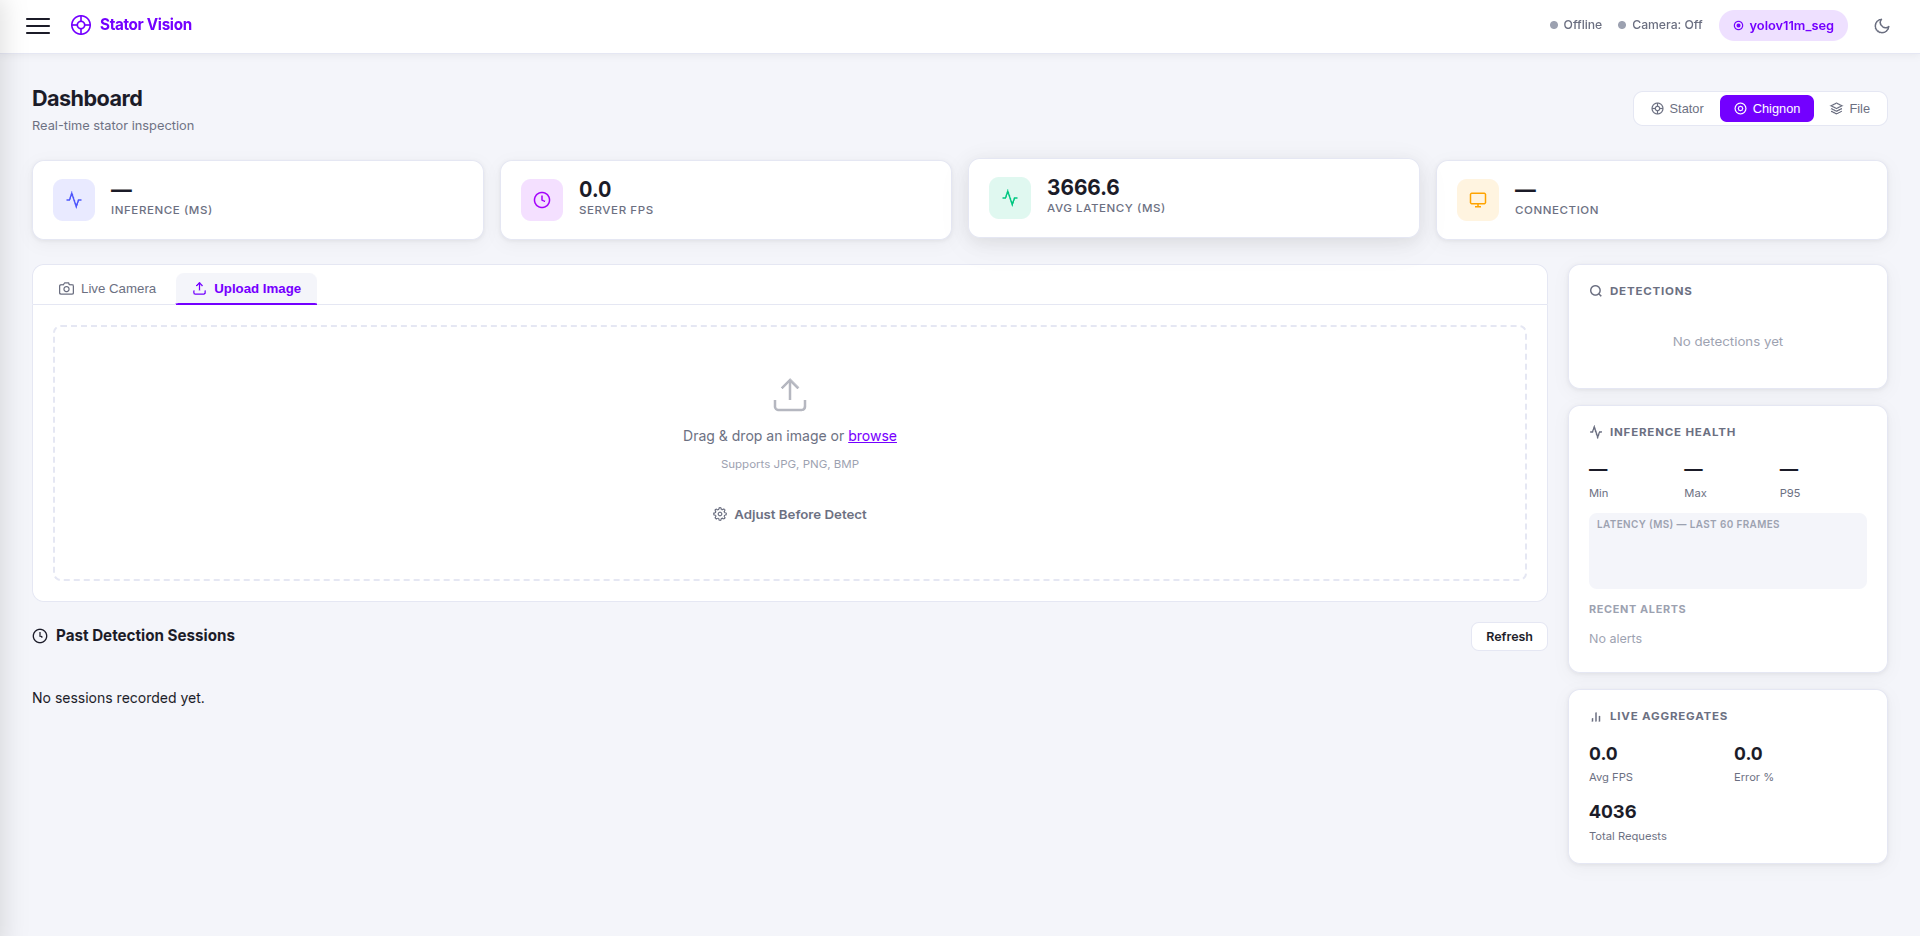
\includegraphics[width=0.95\textwidth]{app_screenshots/dashboard_page.png}
    \caption{\textbf{Tableau de bord principal} --- Vue globale de l'interface utilisateur, incluant la s\'election de domaine, le panneau de configuration, les m\'etriques d'inf\'erence temps r\'eel et la zone de visualisation.}
\end{figure}

\begin{figure}[H]
    \centering
    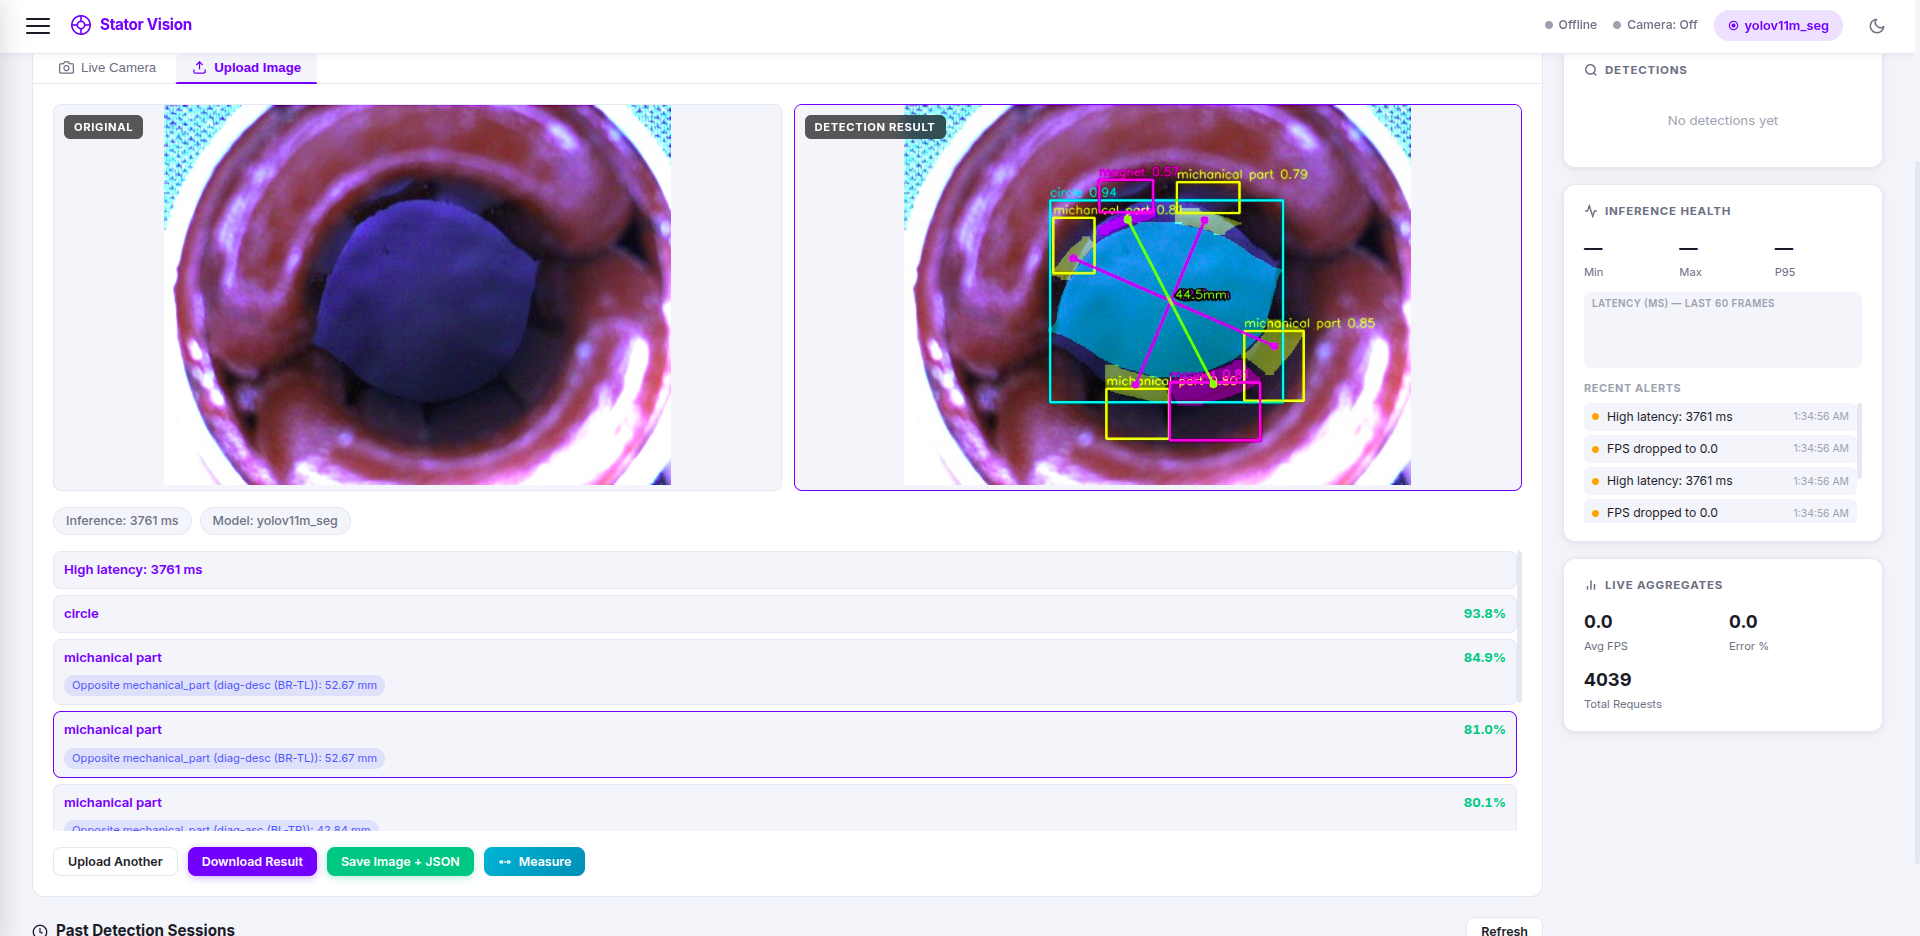
\includegraphics[width=0.95\textwidth]{app_screenshots/dashboard_stator_detection_example_with_cross_diameter_distances.png}
    \caption{\textbf{Inspection Stator (Temps R\'eel)} --- D\'etection des 4 classes avec mesures g\'eom\'etriques dynamiques. Le syst\`eme calcule les dimensions des contours et les distances intra-composants (notamment les distances cross-diam\'etriques) directement sur le flux WebRTC.}
\end{figure}

\begin{figure}[H]
    \centering
    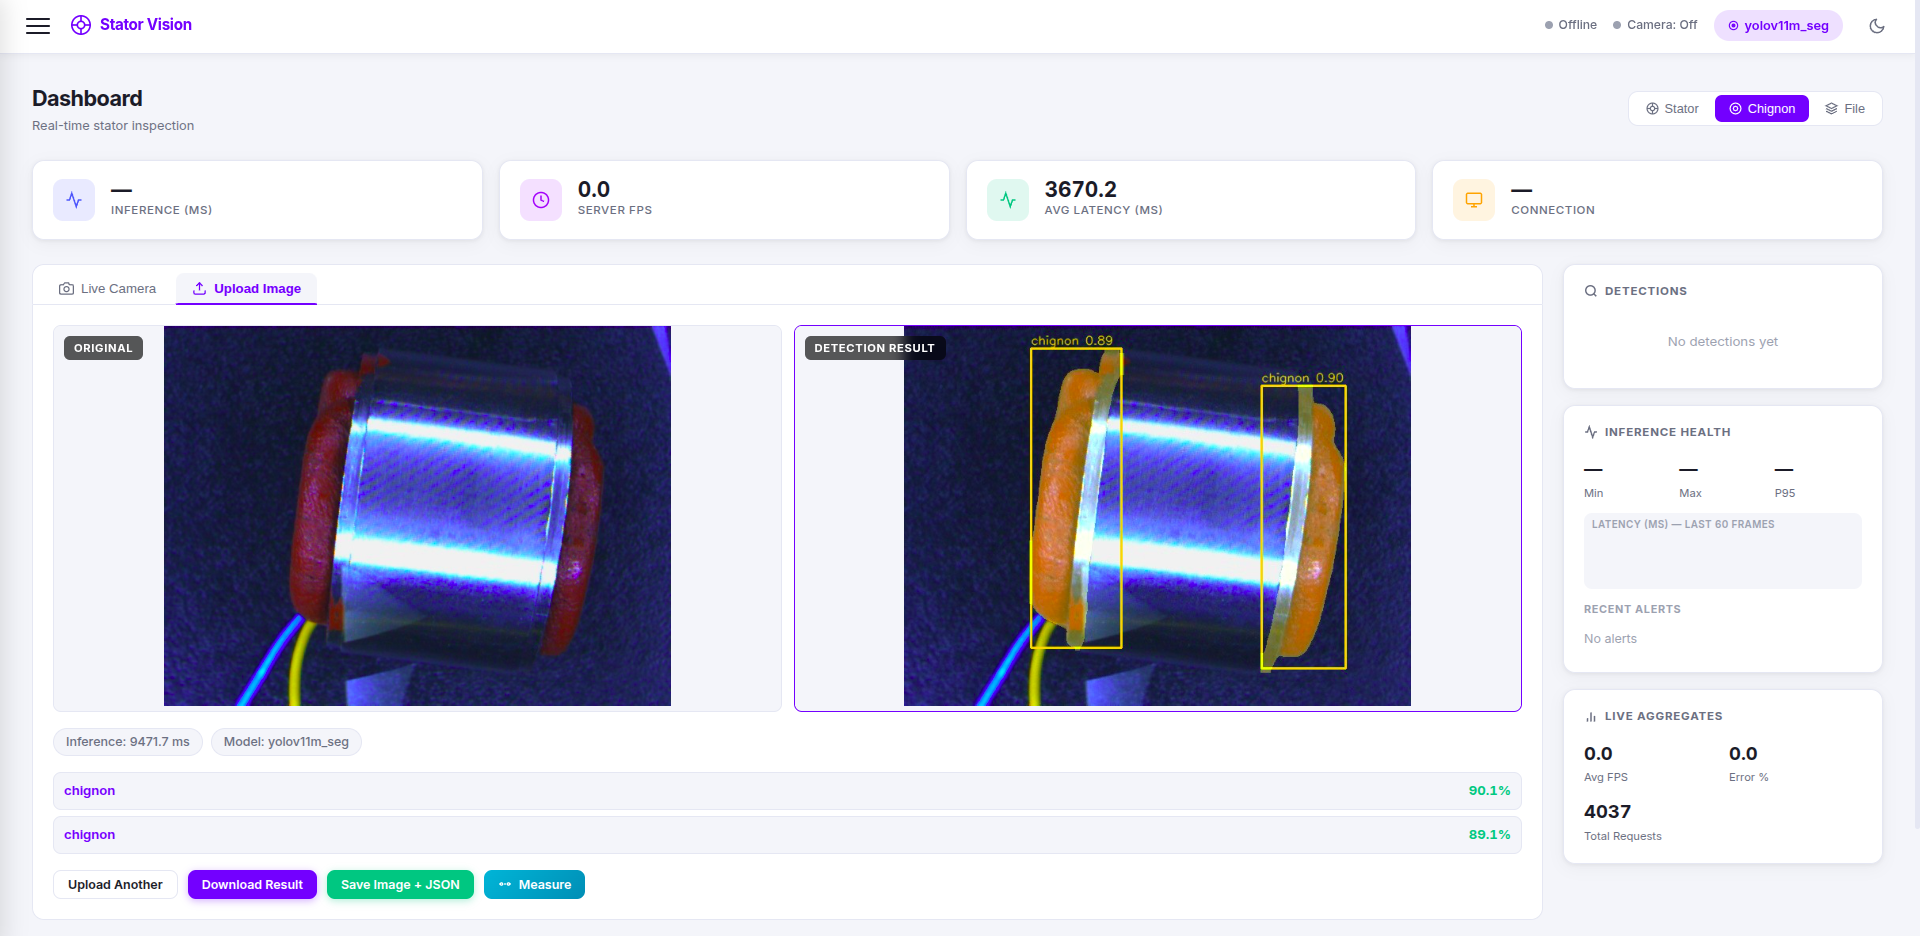
\includegraphics[width=0.95\textwidth]{app_screenshots/dashboard_chignon_detection_example.png}
    \caption{\textbf{Inspection Chignon} --- Segmentation binaire isolant les bobinages de cuivre (coloration verte semi-transparente) via le mod\`ele s\'electionn\'e.}
\end{figure}

\begin{figure}[H]
    \centering
    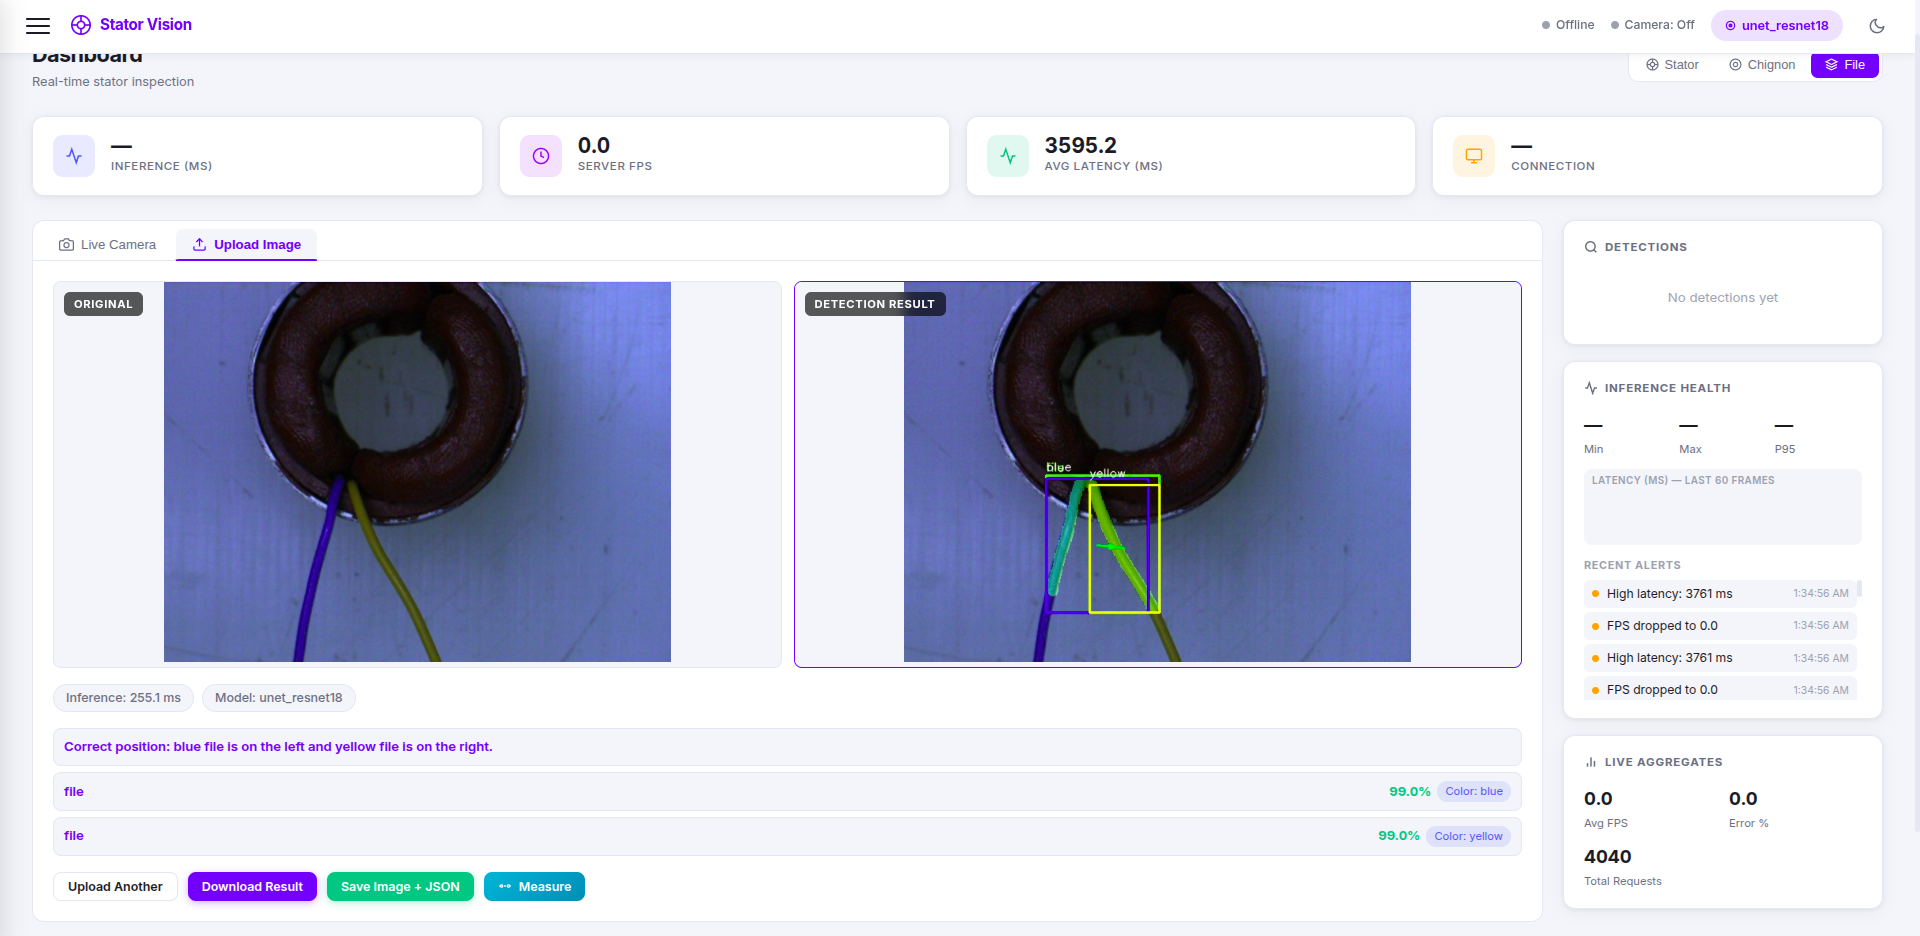
\includegraphics[width=0.95\textwidth]{app_screenshots/dashboard_files_detection_example.png}
    \caption{\textbf{Inspection C\^ables (Files)} --- Segmentation et validation de la conformit\'e couleur (disposition gauche/droite correcte) avec g\'en\'eration d'un statut "OK" sur le panneau de r\'esultats.}
\end{figure}

\begin{figure}[H]
    \centering
    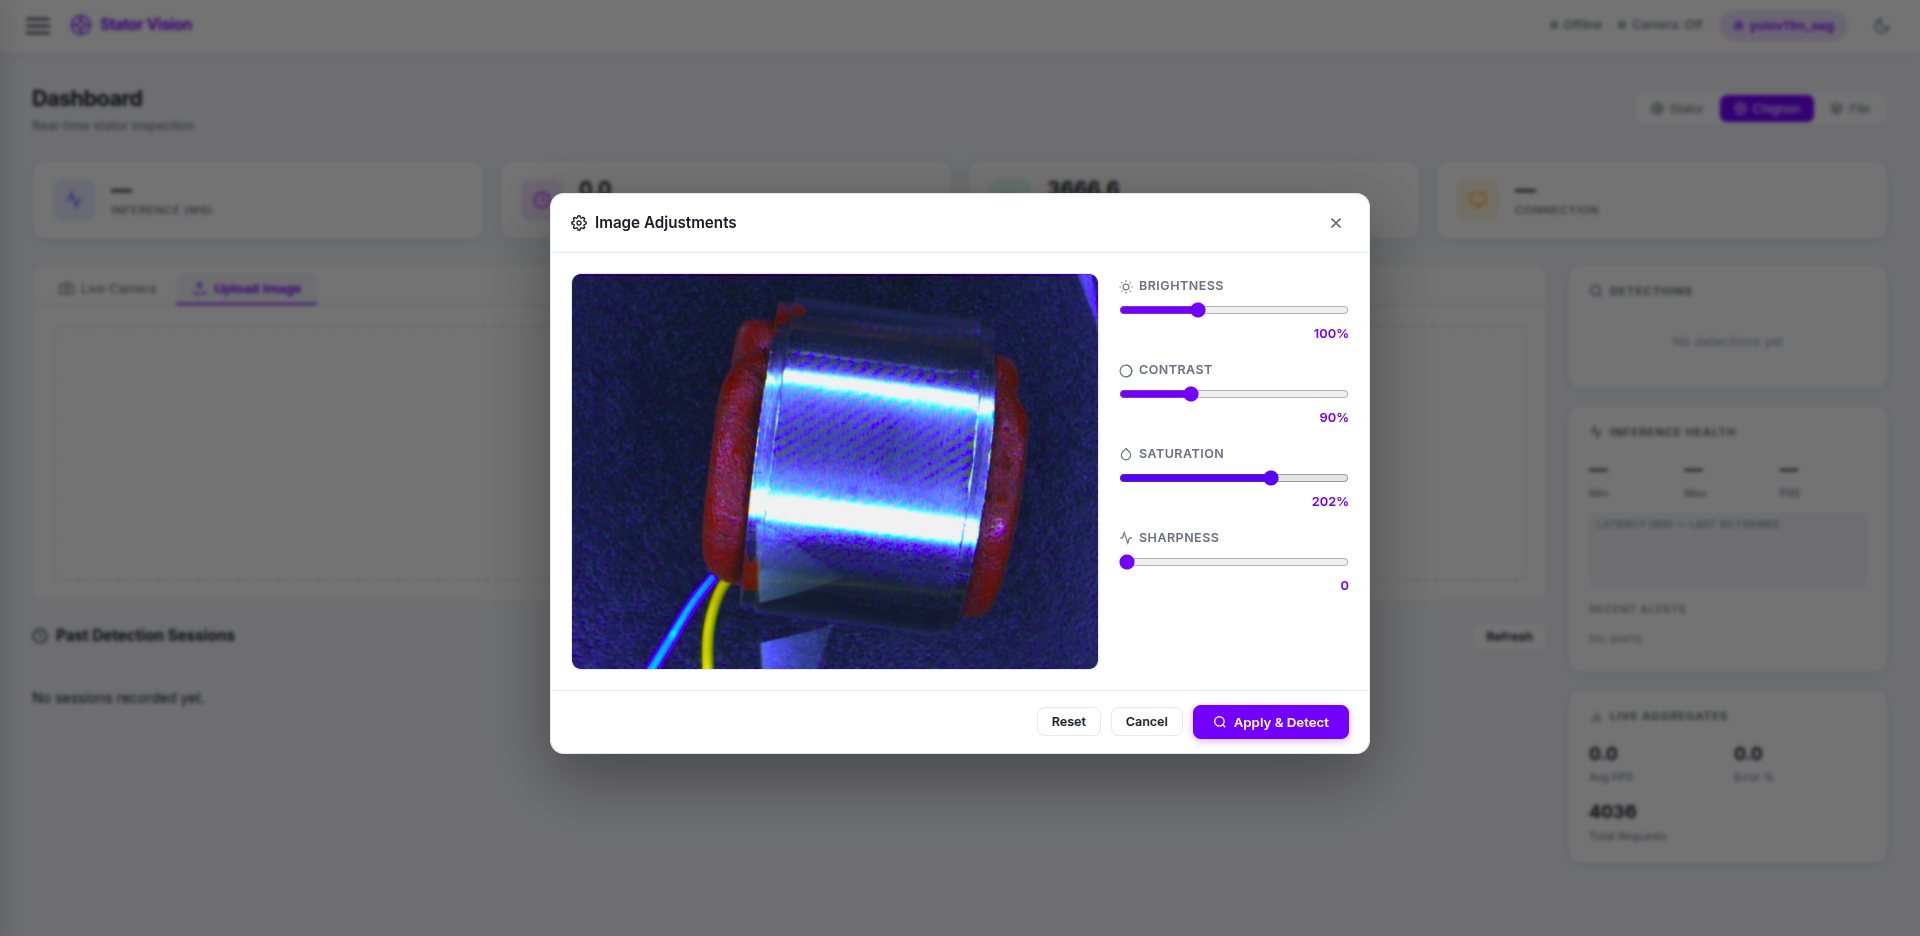
\includegraphics[width=0.95\textwidth]{app_screenshots/edit_contrast_and_brightness_before_detection_chignon_case.png}
    \caption{\textbf{Ajustements photom\'etriques} --- Outils int\'egr\'es permettant \`a l'op\'erateur de modifier la luminosit\'e, le contraste et la saturation de l'image avant l'inf\'erence pour compenser les variations d'\'eclairage.}
\end{figure}

\begin{figure}[H]
    \centering
    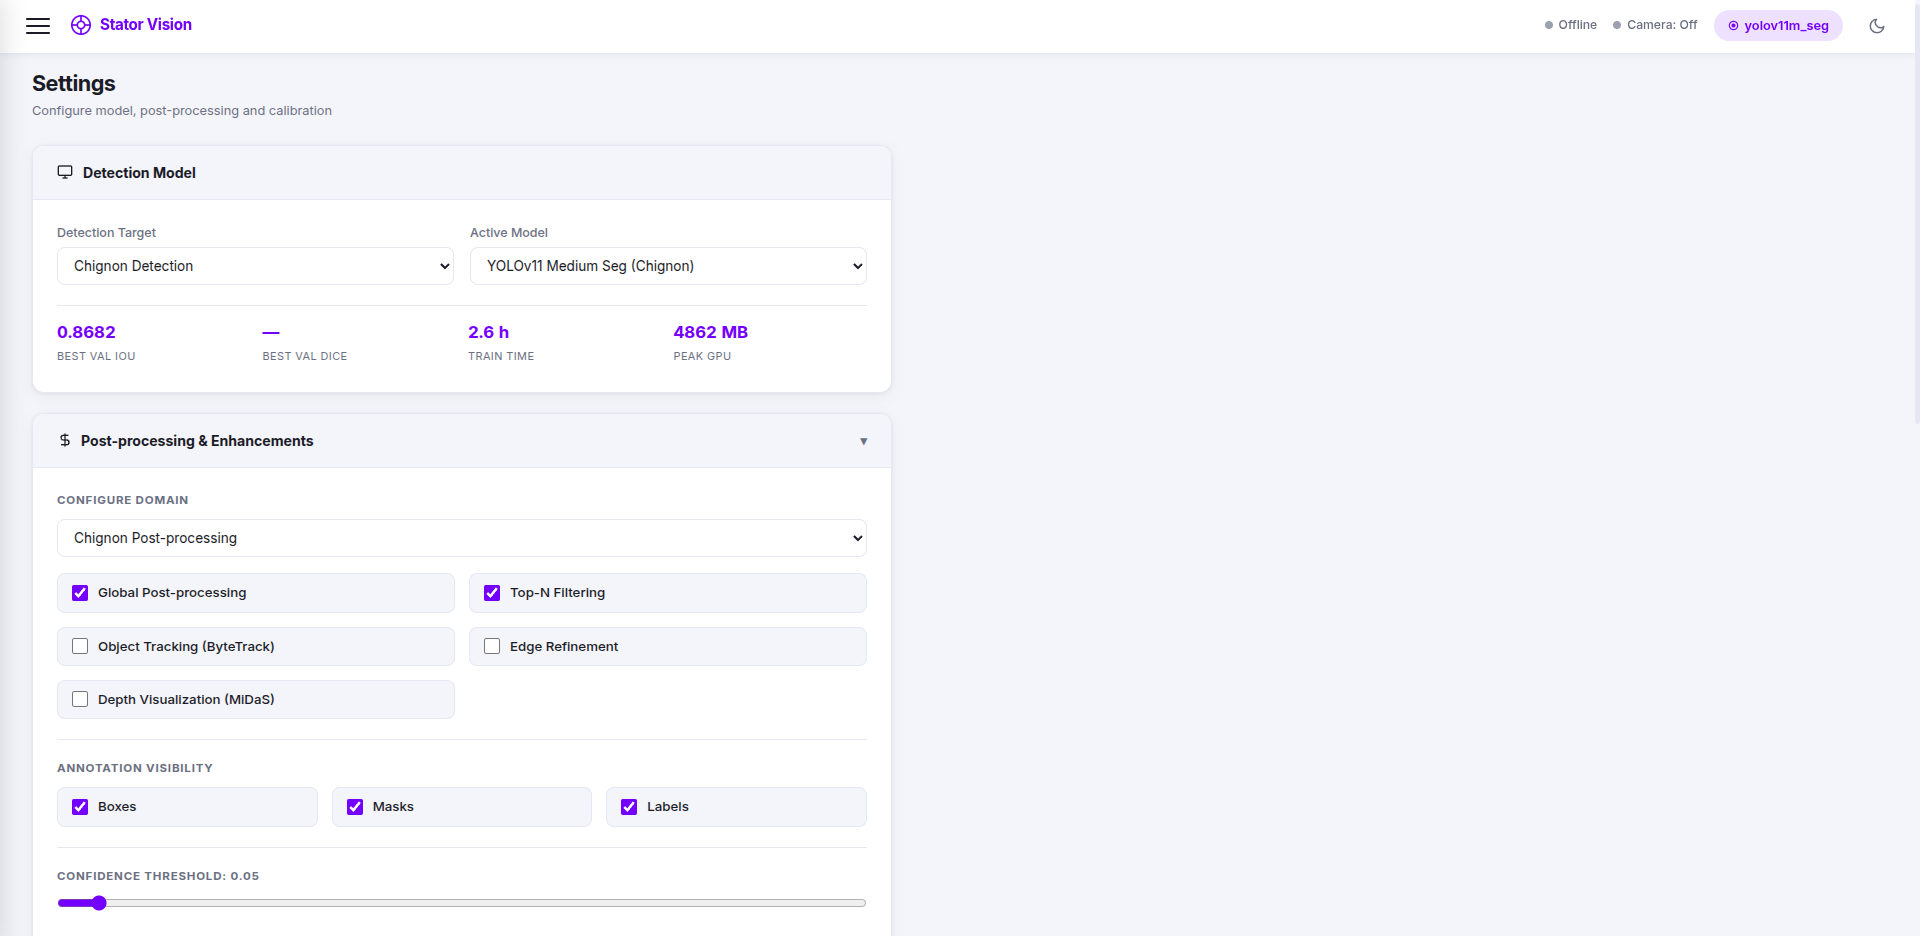
\includegraphics[width=0.95\textwidth]{app_screenshots/settings_page_detection_model_and_postprocessing_methods.png}
    \caption{\textbf{Panneau Mod\`eles \& Intelligence Artificielle} --- S\'election \`a la vol\'ee de l'architecture d'inf\'erence (YOLO, UNet) et activation des filtres de post-traitement avanc\'es (ByteTrack, Guided Filter).}
\end{figure}

\begin{figure}[H]
    \centering
    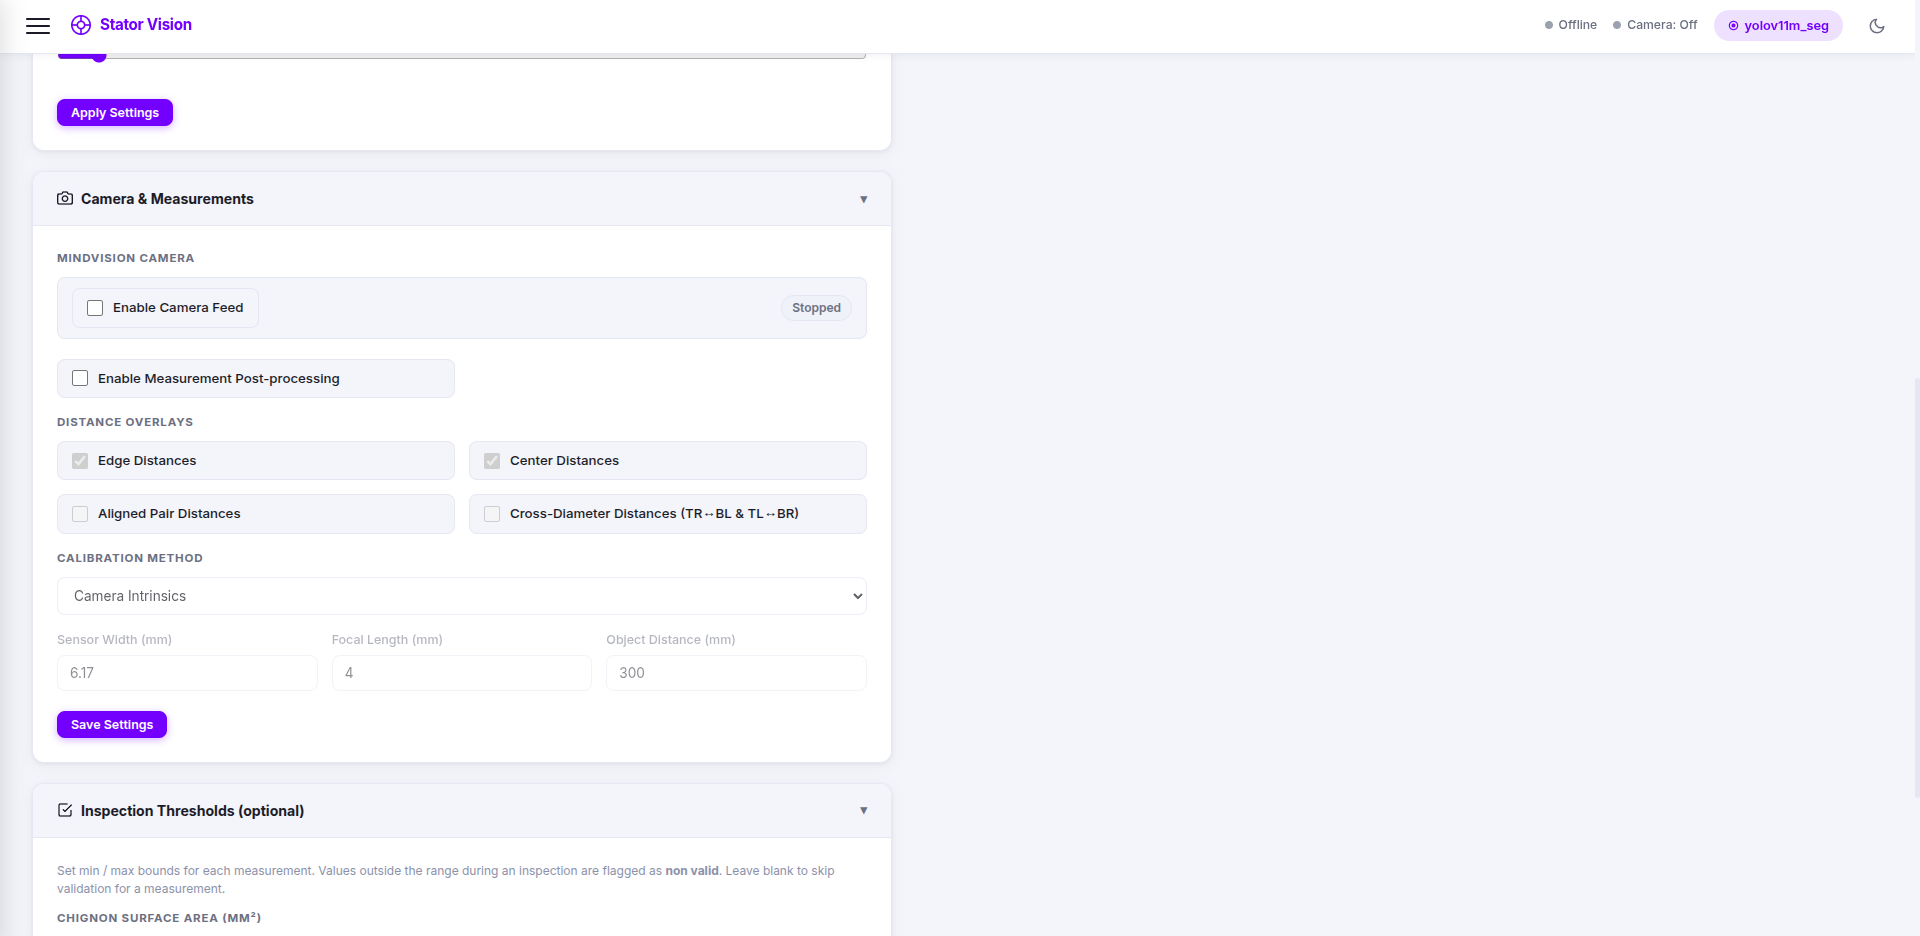
\includegraphics[width=0.95\textwidth]{app_screenshots/settings_camera_and_measurement.png}
    \caption{\textbf{Panneau Cam\'era \& Calibration g\'eom\'etrique} --- S\'election de la source d'entr\'ee (Webcam, Flux HTTP) et configuration de la m\'ethode de calibration (intrins\`eque, label manuel, etc.) pour la conversion des pixels en millim\`etres.}
\end{figure}

\begin{figure}[H]
    \centering
    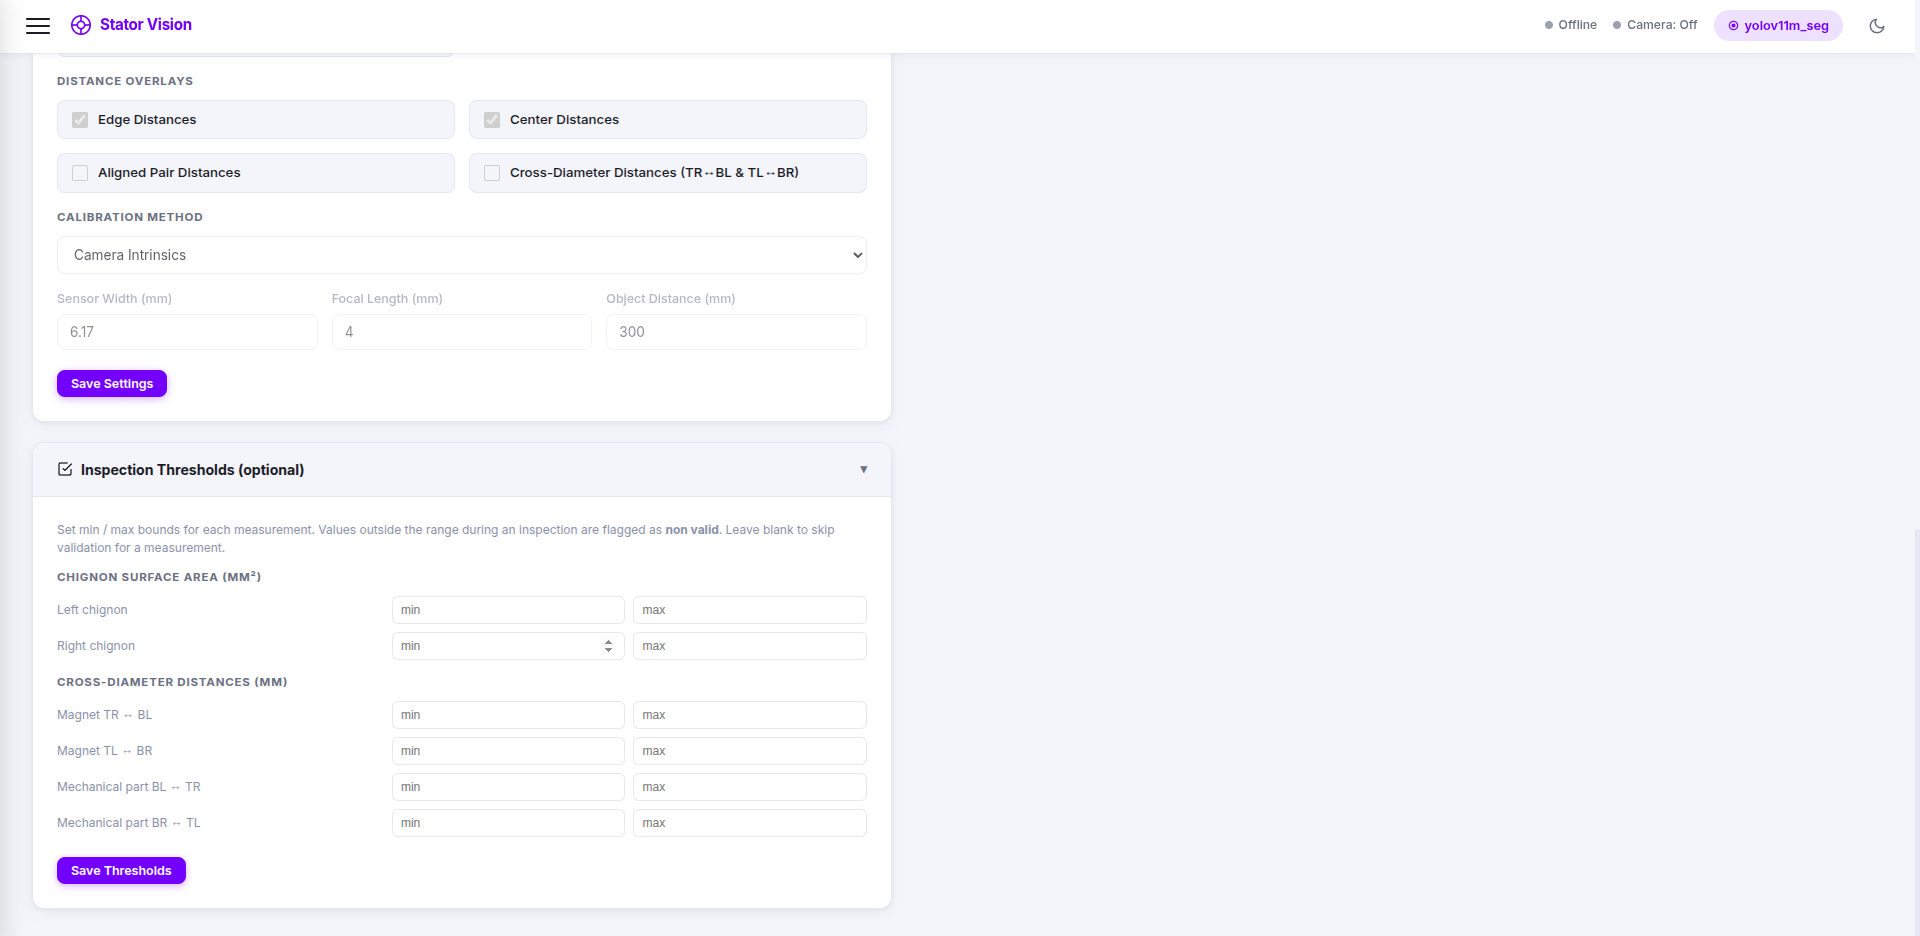
\includegraphics[width=0.95\textwidth]{app_screenshots/setting_inspection_threshould_.png}
    \caption{\textbf{Tol\'erances et r\`egles d'inspection} --- D\'efinition des bornes de d\'ecision (min/max) pour valider automatiquement une pi\`ece. Le syst\`eme inspecte l'aire des chignons gauche/droit et les distances cross-diam\'etriques des p\^oles magn\'etiques et des pi\`eces m\'ecaniques. Toute mesure en dehors des clous d\'eclenche une alerte qualifiante.}
\end{figure}

\begin{figure}[H]
    \centering
    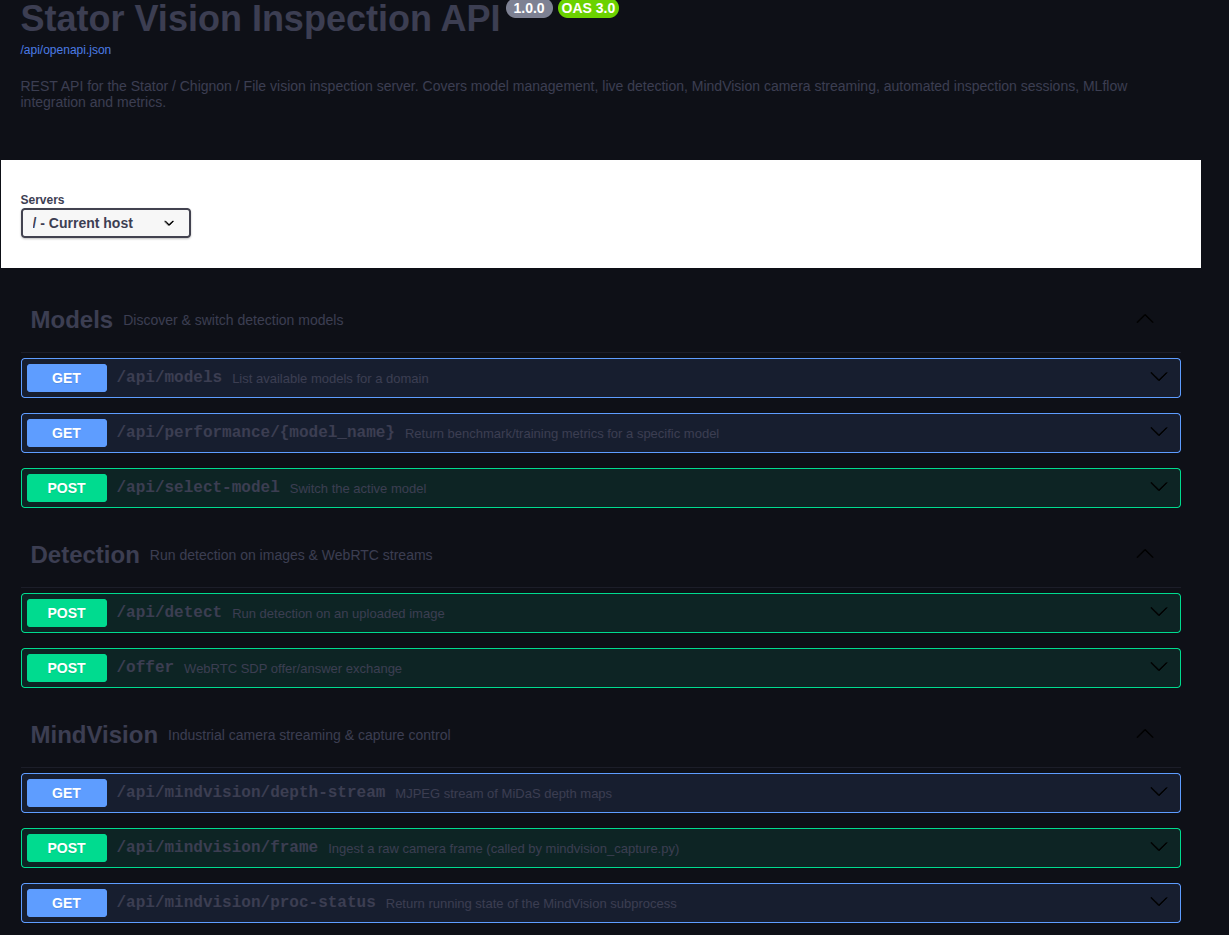
\includegraphics[width=0.95\textwidth]{app_screenshots/swagger_documentation_of_api.png}
    \caption{\textbf{Documentation API Swagger} --- Interface interactive (accessible via le chemin \texttt{/apidocs}) d\'etaillant de fa\c{c}on standardis\'ee l'ensemble des endpoints du backend. L'objectif de cette documentation OpenAPI est de fournir un contrat clair et testable pour permettre une int\'egration fluide et universelle de la solution d'inspection avec des syst\`emes d'usine tiers (automates programmables, bases de donn\'ees qualit\'e d'entreprise, ERP) sans n\'ecessiter d'audit du code h\^ote.}
\end{figure}


% ==========================================================================
\chapter{Optimisations et Am\'eliorations SOTA}
% ==========================================================================

\section{Optimisation de l'inf\'erence}

Plusieurs techniques d'optimisation sont mises en \oe uvre pour maximiser le d\'ebit d'inf\'erence~:

\begin{itemize}
    \item \textbf{FP16 automatique} --- D\'etection du GPU CUDA et conversion en demi-pr\'ecision~: r\'eduit la consommation m\'emoire de $\sim$50\,\% et acc\'el\`ere les calculs sur les Tensor Cores NVIDIA.
    \item \textbf{Compilation JIT} --- Optimisation du graphe de calcul par fusion d'op\'erations pour les mod\`eles PyTorch $\geq 2.x$.
    \item \textbf{ONNX Runtime} --- Support des mod\`eles export\'es au format ONNX avec acc\'el\'eration GPU~: permet l'interop\'erabilit\'e entre frameworks.
    \item \textbf{TensorRT Engine} --- Compilation native pour GPU NVIDIA sp\'ecifique~: optimisation la plus avanc\'ee, avec quantification INT8 optionnelle, offrant les meilleures performances d'inf\'erence en production.
\end{itemize}

\section{Entra\^inement sur Kaggle}

Pour contourner les limitations mat\'erielles locales, un pipeline d'entra\^inement \`a distance est d\'evelopp\'e pour l'environnement Kaggle~:
\begin{itemize}
    \item G\'en\'eration automatique d'un notebook standalone \`a partir du projet
    \item Optimisation VRAM pour GPU P100 (16\,GB) et T4 (15\,GB)~: ajustement automatique de la taille des lots et de la r\'esolution
    \item Gestion automatique des d\'ependances et t\'el\'echargement des jeux de donn\'ees
\end{itemize}


% ==========================================================================
\chapter{Conclusion et Perspectives}
% ==========================================================================

\section{Bilan}

Ce projet a permis de d\'evelopper un syst\`eme complet d'inspection visuelle industrielle couvrant l'ensemble du cycle de vie d'un syst\`eme IA~:

\begin{enumerate}
    \item Un pipeline de donn\'ees robuste avec augmentation $45\times$ incluant la m\'ethode Copy-Paste~\cite{ghiasi2021copypaste}
    \item L'entra\^inement et la comparaison de plus de 9 architectures de segmentation sur 3 domaines, avec des fonctions de perte composites (BCE + Dice + Boundary~\cite{kervadec2019boundary} + Lov\'asz~\cite{berman2018lovasz})
    \item Des r\'esultats d'IoU d\'epassant \textbf{96\,\%} pour les mod\`eles UNet ResNet18~\cite{ronneberger2015unet,he2016resnet}
    \item Un post-traitement intelligent~: heuristique spatiale, filtre Top-N, ByteTrack~\cite{zhang2022bytetrack}, mesures g\'eom\'etriques, MiDaS~\cite{ranftl2020midas}
    \item Une application web temps r\'eel fonctionnelle avec WebRTC, Docker et MLflow
    \item Un syst\`eme de mesure calibr\'e avec 4 m\'ethodes de conversion px$\to$mm
\end{enumerate}

\section{R\'esum\'e des performances}

\begin{table}[H]
\centering
\begin{tabular}{lccc}
\toprule
\textbf{Domaine} & \textbf{Meilleur IoU} & \textbf{Meilleur Mod\`ele} & \textbf{Nb Classes} \\
\midrule
Stator   & 0.9663 & UNet ResNet18~\cite{ronneberger2015unet,he2016resnet}    & 4 \\
Chignon  & 0.9816 & UNet ResNet18~\cite{ronneberger2015unet,he2016resnet}    & 2 \\
Files    & 0.9197 & UNet ResNet18~\cite{ronneberger2015unet,he2016resnet}    & 2 \\
\bottomrule
\end{tabular}
\caption{R\'esum\'e des meilleurs r\'esultats par domaine. UNet ResNet18 domine les trois domaines, confirmant la sup\'eriorit\'e des architectures encodeur-d\'ecodeur sp\'ecialis\'ees dans les r\'egimes de donn\'ees industrielles limit\'ees.}
\end{table}

\section{Perspectives}

\begin{itemize}
    \item \textbf{Int\'egration de YOLOv26}~: Architecture NMS-free avec inf\'erence bout-en-bout pour am\'eliorer les performances YOLO et r\'eduire la latence de post-traitement
    \item \textbf{Cam\'eras haute r\'esolution}~: Test avec des cam\'eras industrielles de r\'esolution $\geq 5$\,Mpx pour am\'eliorer la pr\'ecision des mesures g\'eom\'etriques
    \item \textbf{D\'etection d'anomalies}~: Extension vers la d\'etection de d\'efauts (rayures, d\'eformations, composants manquants) par apprentissage semi-supervis\'e ou auto-supervis\'e
    \item \textbf{D\'eploiement embarqu\'e}~: Portage sur NVIDIA Jetson Orin ou NXP i.MX 8 pour une inspection autonome sans connexion r\'eseau
    \item \textbf{Calibration multi-vue}~: St\'er\'eovision ou lumi\`ere structur\'ee pour des mesures 3D pr\'ecises des stators
    \item \textbf{SegFormer plus large}~: Exp\'erimentation avec SegFormer-B2 ou B4~\cite{xie2021segformer} pour \'evaluer le gain de pr\'ecision contre le co\^ut computationnel
\end{itemize}


% -- Annexes ---------------------------------------------------------------
\appendix

\chapter{Configuration des hyperparam\`etres}
\begin{table}[H]
\centering
\begin{tabular}{ll}
\toprule
\textbf{Hyperparam\`etre} & \textbf{Valeur} \\
\midrule
Taille d'image          & $512 \times 512$ (PyTorch) / $640 \times 640$ (YOLO) \\
Taille des lots         & 4--8 \\
Taux d'apprentissage    & $10^{-4}$ (standard) / $10^{-6}$ (fine-tuning) \\
Optimiseur              & AdamW~\cite{loshchilov2019adamw} \\
Planificateur           & Cosine Annealing / Plateau \\
Arr\^et pr\'ecoce          & Patience 10--30 \'epoques \\
R\'egularisation          & $10^{-4}$ \\
Graine al\'eatoire        & 42 \\
Pr\'ecision               & Mixte (FP16 + FP32) \\
Nombre d'\'epoques max    & 30--50 \\
Split train/val/test    & 70\,\% / 15\,\% / 15\,\% \\
Augmentation            & $45\times$ (g\'eom\'etrique $5\times$ + photom\'etrique $9\times$) \\
Copy-Paste              & Activ\'e~\cite{ghiasi2021copypaste} \\
\bottomrule
\end{tabular}
\caption{Hyperparam\`etres principaux d'entra\^inement}
\end{table}


% ==========================================================================
% BIBLIOGRAPHIE
% ==========================================================================

\begin{thebibliography}{99}

\bibitem{ronneberger2015unet}
O. Ronneberger, P. Fischer, T. Brox,
\textit{U-Net: Convolutional Networks for Biomedical Image Segmentation},
Medical Image Computing and Computer-Assisted Intervention (MICCAI),
Lecture Notes in Computer Science, vol. 9351, pp. 234--241,
Springer, 2015.
\url{https://arxiv.org/abs/1505.04597}

\bibitem{he2016resnet}
K. He, X. Zhang, S. Ren, J. Sun,
\textit{Deep Residual Learning for Image Recognition},
Proceedings of the IEEE Conference on Computer Vision and Pattern Recognition (CVPR),
pp. 770--778, 2016.
\url{https://arxiv.org/abs/1512.03385}

\bibitem{xie2021segformer}
E. Xie, W. Wang, Z. Yu, A. Anandkumar, J. M. Alvarez, P. Luo,
\textit{SegFormer: Simple and Efficient Design for Semantic Segmentation with Transformers},
Advances in Neural Information Processing Systems (NeurIPS), vol. 34,
pp. 12077--12090, 2021.
\url{https://arxiv.org/abs/2105.15203}

\bibitem{chen2017deeplabv3}
L.-C. Chen, G. Papandreou, F. Schroff, H. Adam,
\textit{Rethinking Atrous Convolution for Semantic Image Segmentation},
arXiv preprint arXiv:1706.05587, 2017.
\url{https://arxiv.org/abs/1706.05587}

\bibitem{jocher2023yolov8}
G. Jocher, A. Chaurasia, J. Qiu,
\textit{Ultralytics YOLOv8},
Version 8.0.0, Ultralytics, 2023.
\url{https://github.com/ultralytics/ultralytics}

\bibitem{ghiasi2021copypaste}
G. Ghiasi, Y. Cui, A. Srinivas, R. Qian, T.-Y. Lin, E. D. Cubuk, Q. V. Le, B. Zoph,
\textit{Simple Copy-Paste Is a Strong Data Augmentation Method for Instance Segmentation},
Proceedings of the IEEE/CVF Conference on Computer Vision and Pattern Recognition (CVPR),
pp. 2918--2928, 2021.
\url{https://arxiv.org/abs/2012.07177}

\bibitem{kervadec2019boundary}
H. Kervadec, J. Bouchtiba, C. Desrosiers, E. Granger, J. Dolz, I. Ben Ayed,
\textit{Boundary Loss for Highly Unbalanced Segmentation},
Proceedings of The 2nd International Conference on Medical Imaging with Deep Learning (MIDL),
Proceedings of Machine Learning Research, vol. 102, pp. 285--296, 2019.
\url{https://arxiv.org/abs/1812.07032}

\bibitem{berman2018lovasz}
M. Berman, A. Rannen Triki, M. B. Blaschko,
\textit{The Lov\'asz-Softmax Loss: A Tractable Surrogate for the Optimization of the Intersection-over-Union Measure in Neural Networks},
Proceedings of the IEEE Conference on Computer Vision and Pattern Recognition (CVPR),
pp. 4413--4421, 2018.
\url{https://arxiv.org/abs/1705.08790}

\bibitem{zhang2022bytetrack}
Y. Zhang, P. Sun, Y. Jiang, D. Yu, F. Weng, Z. Yuan, P. Luo, W. Liu, X. Wang,
\textit{ByteTrack: Multi-Object Tracking by Associating Every Detection Box},
European Conference on Computer Vision (ECCV),
Lecture Notes in Computer Science, vol. 13682,
Springer, Cham, pp. 1--21, 2022.
\url{https://arxiv.org/abs/2110.06864}

\bibitem{ranftl2020midas}
R. Ranftl, K. Lasinger, D. Hafner, K. Schindler, V. Koltun,
\textit{Towards Robust Monocular Depth Estimation: Mixing Datasets for Zero-Shot Cross-Dataset Transfer},
IEEE Transactions on Pattern Analysis and Machine Intelligence (TPAMI),
vol. 44, no. 3, pp. 1623--1637, 2022.
\url{https://arxiv.org/abs/1907.01341}

\bibitem{long2015fcn}
J. Long, E. Shelhamer, T. Darrell,
\textit{Fully Convolutional Networks for Semantic Segmentation},
Proceedings of the IEEE Conference on Computer Vision and Pattern Recognition (CVPR),
pp. 3431--3440, 2015.
\url{https://arxiv.org/abs/1411.4038}

\bibitem{loshchilov2019adamw}
I. Loshchilov, F. Hutter,
\textit{Decoupled Weight Decay Regularization},
Proceedings of the International Conference on Learning Representations (ICLR),
2019.
\url{https://arxiv.org/abs/1711.05101}

\bibitem{howard2019mobilenetv3}
A. Howard, M. Sandler, G. Chu, L.-C. Chen, B. Chen, M. Tan, W. Wang, Y. Zhu, R. Pang, V. Vasudevan, Q. V. Le, H. Adam,
\textit{Searching for MobileNetV3},
Proceedings of the IEEE/CVF International Conference on Computer Vision (ICCV),
pp. 1314--1324, 2019.
\url{https://arxiv.org/abs/1905.02244}

\end{thebibliography}

\end{document}